\documentclass[11pt]{article}

% Deterministic PDF metadata for reproducible release builds.
\ifdefined\pdfinfoomitdate\pdfinfoomitdate=1\fi
\ifdefined\pdftrailerid\pdftrailerid{}\fi
\ifdefined\pdfsuppressptexinfo\pdfsuppressptexinfo=15\fi

\usepackage[T1]{fontenc}
\usepackage[utf8]{inputenc}
\usepackage{lmodern}
\usepackage[margin=1in]{geometry}
\usepackage{amsmath,amssymb,amsthm,mathtools,bm,stmaryrd}
\usepackage{booktabs,array,longtable,multirow}
\usepackage{enumitem}
\usepackage{microtype}
\usepackage{xcolor}
\usepackage{hyperref}
\usepackage[nameinlink,noabbrev]{cleveref}
\crefname{lstlisting}{listing}{listings}
\Crefname{lstlisting}{Listing}{Listings}
\usepackage{tikz}
\usetikzlibrary{positioning,calc,arrows.meta,fit,backgrounds}
\usepackage{tikz-cd}
\usepackage{algorithm}
\usepackage{algpseudocode}
\usepackage[most]{tcolorbox}
\usepackage{fancyhdr}
\usepackage{setspace}
\usepackage{listings}
\usepackage{xspace}

\hypersetup{
  colorlinks=true,
  linkcolor=blue!55!black,
  citecolor=green!40!black,
  urlcolor=blue!65!black,
  pdftitle={Operator-Symbolic Languages for Artificial Intelligence - Finite Metatheory Draft v0.5},
  pdfauthor={Komorebi P.},
  pdfsubject={A typed operator-symbolic intermediate language for heterogeneous artificial agents},
  pdfkeywords={operator algebra, neural-symbolic AI, provenance, proof-carrying semantics, latent communication, Komorebi},
  hypertexnames=false
}

\pagestyle{fancy}
\fancyhf{}
\lhead{Operator-Symbolic Languages for AI}
\rhead{Finite Metatheory Draft}
\cfoot{\thepage}
\setlength{\headheight}{14pt}

\newtheorem{theorem}{Theorem}[section]
\newtheorem{proposition}[theorem]{Proposition}
\newtheorem{lemma}[theorem]{Lemma}
\newtheorem{corollary}[theorem]{Corollary}
\newtheorem{conjecture}[theorem]{Conjecture}
\theoremstyle{definition}
\newtheorem{definition}[theorem]{Definition}
\newtheorem{example}[theorem]{Example}
\newtheorem{assumption}[theorem]{Assumption}
\newtheorem{openproblem}[theorem]{Open Problem}
\theoremstyle{remark}
\newtheorem{remark}[theorem]{Remark}

\definecolor{provedgreen}{RGB}{225,245,229}
\definecolor{condblue}{RGB}{228,239,252}
\definecolor{conjorange}{RGB}{255,241,219}
\definecolor{placeholdergray}{RGB}{242,242,242}
\definecolor{warningred}{RGB}{252,231,231}
\definecolor{syntaxviolet}{RGB}{240,234,250}
\definecolor{codegreen}{RGB}{28,110,65}
\definecolor{codegray}{RGB}{92,92,92}
\definecolor{codeblue}{RGB}{28,68,145}
\definecolor{codeorange}{RGB}{170,75,15}

\newtcolorbox{statusbox}{
  breakable,
  colback=condblue,
  colframe=blue!55!black,
  title=Draft status,
  fonttitle=\bfseries
}
\newtcolorbox{provedbox}{
  breakable,
  colback=provedgreen,
  colframe=green!45!black,
  title=Established in this manuscript,
  fonttitle=\bfseries
}
\newtcolorbox{placeholderbox}[1][]{
  breakable,
  colback=placeholdergray,
  colframe=black!45,
  title=Open theory boundary,
  fonttitle=\bfseries,
  #1
}
\newtcolorbox{conjecturebox}{
  breakable,
  colback=conjorange,
  colframe=orange!65!black,
  title=Conjectural extension,
  fonttitle=\bfseries
}
\newtcolorbox{boundarybox}{
  breakable,
  colback=warningred,
  colframe=red!55!black,
  title=Claim boundary,
  fonttitle=\bfseries
}
\newtcolorbox{syntaxbox}{
  breakable,
  colback=syntaxviolet,
  colframe=violet!55!black,
  title=Operator-symbolic expression,
  fonttitle=\bfseries
}

\lstdefinelanguage{OSL}{
  morekeywords={module,lineage,extends,agent,grant,revoke,effect,uses,until,space,dim,vector,in,values,operator,kind,matrix,apply,transport,check_projector,check_intertwiner,between,and,tolerance,observe,infer,simulate,inject,neural_propose,communicate,from,to,as,bind,quarantine,endorse,threshold,authorize,for,proof,mode,persistent,affine,linear,attest,admit,reject_candidate,write_memory,plan,using,expected,execute,feedback,observed,contract,always,after,within,check_contracts,verify_receipts,begin_transaction,commit_transaction,rollback_transaction,session,participants,initial,session_transition,session_terminal,verify_session,start_session,secret,metadata,source,trusted,agent,assert,packet,provenance,accessible_to,quarantined_by,memory,contains,action,executed,approx,parent,show,let,hypotheses,abduct,minimizing,probe,choose_information_gain,risk,repair,validate,transaction,require,else,rollback,modify_model,produces,carries,requires,effects,conf,with},
  sensitive=true,
  morecomment=[l]{\#},
  morestring=[b]",
}
\lstdefinestyle{osl}{
  language=OSL,
  basicstyle=\ttfamily\small,
  keywordstyle=\color{codeblue}\bfseries,
  commentstyle=\color{codegreen},
  stringstyle=\color{codeorange},
  numberstyle=\tiny\color{codegray},
  numbers=left,
  numbersep=7pt,
  showstringspaces=false,
  columns=fullflexible,
  keepspaces=true,
  breaklines=true,
  breakatwhitespace=false,
  frame=single,
  rulecolor=\color{black!25},
  backgroundcolor=\color{black!2},
  tabsize=2,
  xleftmargin=1.2em,
  framexleftmargin=0.8em,
  aboveskip=0.8em,
  belowskip=0.8em,
}

\newcommand{\LangAI}{\mathbb L_{\mathrm{AI}}}
\newcommand{\Lat}{\mathcal H}
\newcommand{\CausalState}{\mathcal X}
\newcommand{\Shared}{\mathcal Z_\star}
\newcommand{\Types}{\mathsf{Types}}
\newcommand{\Terms}{\mathsf{Terms}}
\newcommand{\Ops}{\mathsf{Operators}}
\newcommand{\Forms}{\mathsf{Formulas}}
\newcommand{\Programs}{\mathsf{Programs}}
\newcommand{\Proofs}{\mathsf{Proofs}}
\newcommand{\Sem}[1]{\llbracket #1\rrbracket}
\newcommand{\End}{\operatorname{End}}
\newcommand{\Hom}{\operatorname{Hom}}
\newcommand{\Prov}{\operatorname{Prov}}
\newcommand{\Auth}{\operatorname{Auth}}
\newcommand{\Access}{\operatorname{Access}}
\newcommand{\Origin}{\operatorname{Origin}}
\newcommand{\Valid}{\operatorname{Valid}}
\newcommand{\Bind}{\operatorname{Bind}}
\newcommand{\Use}{\operatorname{Use}}
\newcommand{\Obs}{\operatorname{Obs}}
\newcommand{\Sim}{\operatorname{Sim}}
\newcommand{\Quar}{\operatorname{Quarantine}}
\newcommand{\argmin}{\operatorname*{arg\,min}}
\newcommand{\argmax}{\operatorname*{arg\,max}}
\newcommand{\RRCT}{\textsc{RRCT}}
\newcommand{\Komorebi}{\textsc{Komorebi}}
\newcommand{\Jspace}{\mathcal J}
\newcommand{\Effects}{\mathsf{Effects}}
\newcommand{\Eff}{\operatorname{Eff}}
\newcommand{\Sig}{\operatorname{Sig}}
\newcommand{\Lip}{\operatorname{Lip}}
\newcommand{\supp}{\operatorname{supp}}
\newcommand{\Cut}{\operatorname{Cut}}
\newcommand{\MergeIdx}{\mathfrak M}
\newcommand{\defect}{\operatorname{def}}
\newcommand{\TODO}[1]{\textcolor{red!70!black}{\textbf{[TODO: #1]}}}
\newcommand{\eps}{\varepsilon}
\newcommand{\OSLCore}{\textnormal{\textsc{OSL-Core}}\xspace}
\newcommand{\OSLIR}{\textnormal{\textsc{OSL-IR}}\xspace}

\title{\textbf{Operator-Symbolic Languages for Artificial Intelligence}\\[0.35em]
\large Geometry, Proof-Carrying Semantics, and Shared Algebraic Communication}
\author{Komorebi P.}
\date{Finite metatheory and independent-kernel draft v0.5}

\begin{document}
\maketitle

\begin{abstract}
We develop an operator-symbolic language as a candidate machine-native intermediate representation for artificial intelligence and introduce \OSLCore, a concrete executable subset. The central thesis is that continuous latent geometry, typed operators, symbolic relations, effect annotations, proof objects, and provenance can be combined into one language in which states function as nouns, operators as verbs, types as grammatical categories, logic as admissibility syntax, causal consequences as semantics, and proof paths as explanations. Distinct models need not share coordinates: they may share an abstract transformation algebra realized through different latent representations and connected by exact or approximate intertwiners. We define the language family \(\LangAI\), give denotational, dynamic, graded, coalgebraic, and effect semantics, and then fix a concrete surface grammar with agents, lineages, vector spaces, projectors, coordinate transport, provenance-aware packets, communication, quarantine, endorsement, memory, planning, capabilities, feedback, assertions, and canonical receipts. Version 0.3 adds linear and affine proof resources, append-only audit semantics, statement-boundary receipts, deterministic semantic replay, finite session-graph verification, explicit-flow analysis, an independent receipt kernel, and two exhaustive finite transition-model layers. The packaged evidence comprises sixty-six source programs, two paired public-projection audits, sixty-one focused tests, 1,149 independently reconstructed receipts, seventy proof terms, 2,330 exhaustively reached abstract states, and 47,958 finite transition checks. Within a finite-dimensional base theory we prove preservation of polynomial operator semantics, approximate relation bounds, coordinate invariance, finite recovery of observational congruences, quotient emergence of symbols, geometric realization of an ordered logical fragment, stability of graded formulas, content-only ownership impossibility, proof-gated execution safety, proof transport, packet block identities, exact interlingua factorization, private closure under channel cuts, finite metadata-capacity bounds, tensor-product preservation, finite-horizon nonlinear transport, effect confinement, and finite-core provenance non-forging. The new computer-assisted results establish the declared finite properties of the abstract kernels and receipt semantics, but do not constitute a proof-assistant verification of the complete interpreter. No claim concerning subjective experience is made.
\end{abstract}

\begin{statusbox}
Version 0.5 consolidates the concrete language as \OSLCore\ 0.3. It preserves the typed AST, proof-gated memory and planning, bounded capabilities, contracts, rollback, sessions, neural proposal quarantine, and metadata audits of version 0.2, while adding resource-sensitive proofs, an append-only audit chain, semantic source-boundary receipts, exact replay certificates, verified finite session graphs, static explicit-flow certificates, an independent receipt/proof kernel, and two complete finite transition-model explorations. Sixty-six source programs and sixty-one focused tests pass their declared specifications. Exact finite results are stated with their model and trust boundaries; approximate and nonlinear claims retain error bounds or open-theory labels. A proof-assistant formalization of the complete syntax and runtime remains open.
\end{statusbox}

\begin{boundarybox}
The framework concerns representations, transformations, proof, provenance, communication, and control. It does not establish consciousness, sentience, personhood, valence, or moral status. A system may implement every formal construction in this paper without possessing subjective experience.
\end{boundarybox}

\tableofcontents
\newpage

\section{Introduction}

\subsection{The language problem for artificial agents}

Artificial agents already manipulate high-dimensional internal states, transform them through learned operators, exchange messages, update memories, and select actions. Yet the representational levels used for these functions are often separated:
\begin{itemize}[leftmargin=1.6em]
  \item neural activations carry continuous information but are difficult to inspect;
  \item symbolic structures are inspectable but often brittle under noise and novel inputs;
  \item natural language is expressive but ambiguous and weakly typed;
  \item action policies are executable but usually do not carry their own provenance or proof.
\end{itemize}

We ask whether these layers can be unified by a machine-native intermediate language whose primitive objects are not merely words, propositions, or vectors, but \emph{typed transformations of structured states}. The motivating slogan is:
\begin{equation}
\boxed{
\begin{aligned}
\text{continuous geometry}
&\longrightarrow
\text{typed operator algebra}\\
&\longrightarrow
\text{symbolic logic and proof}
\longrightarrow
\text{language or action}.
\end{aligned}
}
\label{eq:stack}
\end{equation}

The proposal does not require neural geometry to disappear. Instead, symbolic expressions name and constrain reusable operator patterns discovered in continuous representations.

\subsection{States, operators, and proof paths}

A latent state is a candidate noun. An operator is a candidate verb. A type specifies the admissible input and output roles. A formula expresses a relation that must hold. A proof term certifies that an inference or operation is authorized. A causal consequence supplies semantics by testing whether the transformation behaves as predicted.

The intended interpretation is summarized by:
\begin{center}
\begin{tabular}{ll}
\toprule
Language-like role & Computational realization \\
\midrule
Noun & state, packet, memory, object, distribution \\
Verb & operator, transition, transport, update \\
Type & admissible role or interface \\
Syntax & composition and logical well-formedness \\
Semantics & causal effect and denotation \\
Authorship & provenance and lineage \\
Explanation & proof path and receipt chain \\
Discourse through time & recurrence and memory update \\
\bottomrule
\end{tabular}
\end{center}

\subsection{Why natural language is not enough}

Natural language is valuable as a human interface, but it is usually:
\begin{itemize}[leftmargin=1.6em]
  \item ambiguous;
  \item context-sensitive;
  \item difficult to execute directly;
  \item weak at representing provenance and authorization;
  \item difficult to verify mechanically;
  \item vulnerable to hidden or unintended side channels.
\end{itemize}
An operator-symbolic intermediate representation can instead be typed, compositional, executable, uncertainty-aware, provenance-preserving, and machine-checkable.

\subsection{Main contributions}

The paper develops the following components:
\begin{enumerate}[leftmargin=1.7em]
  \item a typed operator-symbolic language \(\LangAI\) with terms, formulas, programs, proof terms, and effects;
  \item denotational, operational, graded, causal, and effect semantics over latent state spaces;
  \item a coordinate-free notion of meaning through operator algebras, presentations, and intertwiners;
  \item finite observational recovery of operator congruences and quotient symbols;
  \item geometric realizations of order, negation, and conjunction without assuming Boolean collapse;
  \item provenance-sensitive, resource-aware, and proof-carrying assertions and actions;
  \item probabilistic and paraconsistent logical states with quantitative stability bounds;
  \item proof translation between heterogeneous symbolic calculi under explicit rule-preservation conditions;
  \item shared algebraic communication among heterogeneous models, with operational criteria for private versus group-level closure;
  \item Komorebi-style packet analysis, transfer blocks, synthesis, residuals, and holonomy;
  \item nonlinear, tensor, manifold, Koopman, kernel, and tensor-network extensions;
  \item a compiler architecture with effect confinement and verification-condition generation;
  \item explicit experiments, baseline families, falsification criteria, and theorem-status boundaries.
\end{enumerate}

\section{Architectural overview}

\subsection{Four representational layers}

We distinguish four coupled layers.

\paragraph{Latent substrate.}
Continuous states:
\[
h_t\in\Lat,
\qquad
x_t\in\CausalState,
\]
may be vectors, tensors, graphs, probability distributions, neural activations, or manifold-valued states.

\paragraph{Operator layer.}
Typed maps act on states:
\[
P_Sx,
\qquad
P_Jh,
\qquad
T_{A\to B}h,
\qquad
F(x,a),
\qquad
R(P_Jh).
\]
These operators perform selection, transport, prediction, reconstruction, and update.

\paragraph{Symbolic layer.}
Typed predicates and modalities express access, belief, provenance, ownership, authorization, and causal use.

\paragraph{Interface layer.}
Natural language, code, diagrams, plans, and physical actions render or execute the internal operator-symbolic state.

\begin{figure}[ht]
\centering
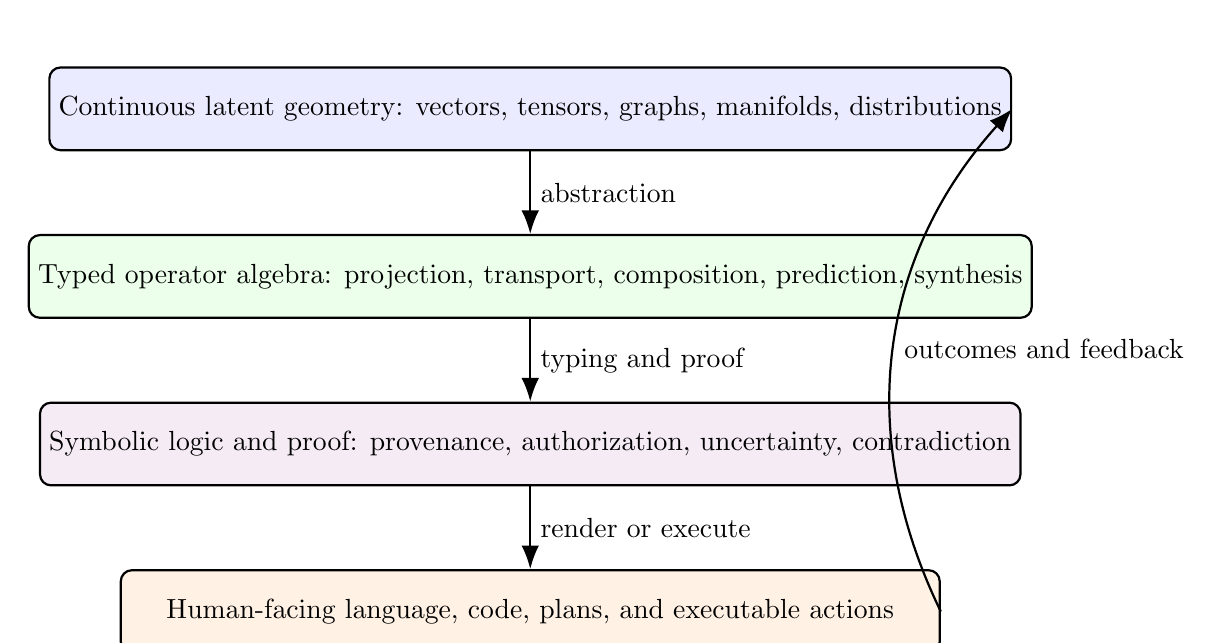
\begin{tikzpicture}[
  node distance=1.05cm,
  box/.style={draw, rounded corners, minimum width=10.4cm, minimum height=1.05cm, align=center, thick},
  arr/.style={-{Latex[length=3mm]}, thick}
]
\node[box, fill=blue!8] (latent) {Continuous latent geometry: vectors, tensors, graphs, manifolds, distributions};
\node[box, fill=green!8, below=of latent] (ops) {Typed operator algebra: projection, transport, composition, prediction, synthesis};
\node[box, fill=violet!8, below=of ops] (logic) {Symbolic logic and proof: provenance, authorization, uncertainty, contradiction};
\node[box, fill=orange!10, below=of logic] (interface) {Human-facing language, code, plans, and executable actions};
\draw[arr] (latent) -- node[right]{abstraction} (ops);
\draw[arr] (ops) -- node[right]{typing and proof} (logic);
\draw[arr] (logic) -- node[right]{render or execute} (interface);
\draw[arr, bend left=34] (interface.east) to node[right]{outcomes and feedback} (latent.east);
\end{tikzpicture}
\caption{The proposed operator-symbolic stack. The feedback arrow is essential: causal consequences revise latent geometry, operators, and symbolic beliefs.}
\label{fig:stack}
\end{figure}

\subsection{The hybrid thesis}

The proposal is not that symbolic logic should replace representation learning. The intended architecture is:
\begin{equation}
\boxed{
\text{latent learning}
\leftrightarrow
\text{operator intermediate representation}
\leftrightarrow
\text{symbolic proof layer}.
}
\label{eq:hybrid}
\end{equation}
The latent layer handles approximation and novelty. The operator layer makes transformations reusable and transportable. The symbolic layer constrains inference, memory, communication, and action.

\subsection{Design axioms}

The framework is organized around six design axioms.
\begin{enumerate}[leftmargin=1.7em,label=\textbf{A\arabic*.}]
  \item \textbf{Gauge tolerance.} Meaning is attached to operator relations and causal roles, not privileged coordinates.
  \item \textbf{Compositionality.} The semantics of a well-typed composite is determined by the semantics of its parts and their composition law.
  \item \textbf{Causal grounding.} Declared meanings must predict intervention-sensitive consequences, not merely correlate with labels.
  \item \textbf{Proof-carrying use.} Memory writes, tool calls, and high-impact actions require typed evidence satisfying declared preconditions.
  \item \textbf{Provenance conservation.} Communication may grant access to content without fabricating direct observation or ownership.
  \item \textbf{Calibrated incompleteness.} When available evidence does not identify one semantics, the language must preserve conflict or abstain rather than force a symbol.
\end{enumerate}

These axioms deliberately separate representation learning from authorization. A learned latent state may propose an operator-symbolic interpretation; the verifier decides which consequences that interpretation is permitted to have.

\section{Mathematical preliminaries}

\subsection{Typed spaces and maps}

Let \(\mathsf T\) be a collection of types. Each type \(\tau\in\mathsf T\) is interpreted as a space:
\[
\Sem{\tau}=X_\tau.
\]
For the finite base theory, each \(X_\tau\) is a finite-dimensional real Hilbert space. More general interpretations are introduced later.

A typed operator symbol
\[
g:\tau\to\sigma
\]
is interpreted as a map
\[
\Sem{g}:X_\tau\to X_\sigma.
\]
Composition is type checked:
\[
g:\tau\to\sigma,
\qquad
f:\sigma\to\upsilon
\quad\Longrightarrow\quad
f\circ g:\tau\to\upsilon.
\]

\subsection{Operator algebras}

Let \(\mathcal A\) be an abstract algebra generated by primitive operations \(\mathcal G\). An agent \(a\) realizes \(\mathcal A\) through a representation
\[
\rho_a:\mathcal A\to\End(\Lat_a).
\]
When \(\mathcal A\) is a monoid algebra, the representation satisfies
\[
\rho_a(g_2g_1)=\rho_a(g_2)\rho_a(g_1),
\qquad
\rho_a(e)=I.
\]
Approximate representations permit bounded residuals.

\subsection{Programs and transitions}

A program \(\alpha\) denotes a transition relation
\[
\Sem{\alpha}\subseteq\mathcal S\times\mathcal S
\]
or, in deterministic settings, a map \(\Sem{\alpha}:\mathcal S\to\mathcal S\). Sequential composition satisfies
\[
\Sem{\alpha;\beta}
=
\Sem{\beta}\circ\Sem{\alpha}.
\]

\subsection{Proof objects}

A proof judgment has the form
\[
\Gamma;\Pi\vdash\varphi,
\]
where \(\Gamma\) is a type and term environment and \(\Pi\) is a provenance and authorization context. A proof term \(p\) inhabits a proposition type:
\[
p:\varphi.
\]
This Curry--Howard-style notation is used operationally: actions may require proof terms before execution.

\section{Definition of the AI-native language}

\begin{definition}[Operator-symbolic AI language]
An operator-symbolic AI language is a tuple
\[
\LangAI
=
(\Types,\Terms,\Ops,\Forms,\Programs,\Proofs,\Effects,\vdash,\Sem{\cdot})
\]
consisting of types, terms, typed operators, formulas, executable programs, proof terms, effect annotations, derivability rules, and semantics.
\end{definition}

\subsection{Core types}

A minimal type system contains:
\begin{center}
\begin{tabular}{lll}
\toprule
Type & Intended denotation & Example inhabitant \\
\midrule
\texttt{State} & causal or latent state & \(x_t\) \\
\texttt{Workspace} & accessible packet state & \(j_t\) \\
\texttt{Agent} & agent identity or interface & \(a\) \\
\texttt{Lineage} & temporal or causal lineage & \(L_a\) \\
\texttt{Memory} & stored event or model & \(m\) \\
\texttt{Observation} & externally grounded event & \(o\) \\
\texttt{Simulation} & internally generated event & \(d\) \\
\texttt{Action} & executable intervention & \(u\) \\
\texttt{Proof} & authorization evidence & \(p\) \\
\texttt{Probability} & calibrated uncertainty & \(q\in[0,1]\) \\
\texttt{Provenance} & source and origin status & \(\rho\) \\
\texttt{Receipt} & proof-carrying transition record & \(r\) \\
\texttt{Channel} & typed communication interface & \(\chi\) \\
\texttt{Effect} & externally visible capability & \(\mathsf{write},\mathsf{act}\) \\
\bottomrule
\end{tabular}
\end{center}

\subsection{Terms}

Terms are generated by
\[
t::=x\mid c\mid g(t)\mid f(t_1,\ldots,t_n)\mid\operatorname{Source}(t)\mid\operatorname{Lineage}(t).
\]
Representative operator terms include
\[
P_S(t),
\qquad
P_J(t),
\qquad
T_{A\to B}(t),
\qquad
\operatorname{Memory}(t),
\qquad
\operatorname{Predict}(t,a).
\]

\subsection{Formulas}

The formula grammar is
\[
\begin{aligned}
\varphi::={}&p(t_1,\ldots,t_n)
\mid\neg\varphi
\mid\varphi\wedge\psi
\mid\varphi\vee\psi
\mid\varphi\to\psi\\
&\mid J_a\varphi
\mid B_{a,L}\varphi
\mid O_a^\kappa\varphi
\mid K_a^q\varphi
\mid U_a\varphi
\mid Q_a\varphi
\mid[\alpha]\varphi
\mid X\varphi.
\end{aligned}
\]
The modalities mean:
\begin{center}
\begin{tabular}{ll}
\toprule
Expression & Meaning \\
\midrule
\(J_a\varphi\) & \(\varphi\) is accessible to agent \(a\) \\
\(B_{a,L}\varphi\) & \(\varphi\) is bound to agent \(a\) under lineage \(L\) \\
\(O_a^\kappa\varphi\) & \(\varphi\) is autobiographically typed by provenance \(\kappa\) \\
\(K_a^q\varphi\) & \(a\) endorses \(\varphi\) with confidence \(q\) \\
\(U_a\varphi\) & \(\varphi\) is causally used in planning \\
\(Q_a\varphi\) & \(\varphi\) is quarantined \\
\([\alpha]\varphi\) & after every execution of \(\alpha\), \(\varphi\) holds \\
\(X\varphi\) & \(\varphi\) holds in the next state \\
\bottomrule
\end{tabular}
\end{center}

\subsection{Programs}

Programs are generated by
\[
\begin{aligned}
\alpha::={}&
\operatorname{sense}
\mid\operatorname{bind}
\mid\operatorname{infer}
\mid\operatorname{plan}
\mid\operatorname{act}
\mid\operatorname{update}\\
&\mid\operatorname{communicate}(\chi,t)
\mid\operatorname{writeMemory}(t)
\mid\operatorname{simulate}(\alpha)
\mid\alpha;\beta\\
&\mid\operatorname{if}\ \varphi\ \operatorname{then}\alpha\ \operatorname{else}\beta.
\end{aligned}
\]

\subsection{Proof terms}

Proof terms may include:
\[
p::=
\operatorname{obsToken}(e)
\mid\operatorname{originToken}(a,e)
\mid\operatorname{lineageToken}(L,e)
\mid\operatorname{authToken}(\alpha)
\mid\operatorname{compose}(p_1,p_2).
\]

\subsection{Effect judgments}

A program judgment has the form
\[
\Gamma;\Pi\vdash
\alpha:\tau\rightsquigarrow\sigma\;!\;\mathcal E,
\]
where \(\mathcal E\subseteq\Effects\) is the set of externally visible effects that the program may emit. Representative effects include
\[
\mathsf{read},\quad
\mathsf{writeMemory},\quad
\mathsf{communicate},\quad
\mathsf{toolCall},\quad
\mathsf{externalAct},\quad
\mathsf{simulate}.
\]
Sequential composition unions effects, while a capability proof may reduce an abstract requested effect to a narrower authorized effect.

\section{OSL-Core: a concrete operator-symbolic language}
\label{sec:osl-core}

The preceding definition describes a family of languages.  This section fixes a
small concrete member of that family, called \OSLCore.  Its purpose is not to
replace neural computation or to settle every metatheoretic question.  It is a
reference intermediate language in which operator declarations, provenance,
proof obligations, memory writes, communication, effects, and action
authorization can be stated in one typed program.

\begin{statusbox}
The release accompanying this manuscript includes a deterministic reference
interpreter for a finite subset, sixty-six source programs, sixty-one automated tests,
and a machine-readable example-suite result.  The interpreter implements the
operational policies described below for finite arrays, provenance-aware
packets, first-class proofs, bounded capabilities, temporal contracts,
transactions, session protocols, neural proposals, memory writes, planning,
effects, and receipts.  It does not implement
the complete higher-order, stochastic, nonlinear, or proof-assistant semantics
proposed elsewhere in the paper.
\end{statusbox}

\subsection{Design goals}

\OSLCore is designed around twelve requirements.
\begin{enumerate}[leftmargin=1.7em]
  \item \textbf{Typed operator composition.}  States and transformations carry
  explicit source and target types.
  \item \textbf{Coordinate tolerance.}  Meaning may be preserved by an
  intertwiner or transported operator even when concrete vectors differ.
  \item \textbf{Provenance conservation.}  Communication preserves source and
  lineage rather than converting foreign content into direct observation.
  \item \textbf{Linear evidence resources.}  Observation and authorization
  tokens cannot be silently forged or duplicated.
  \item \textbf{Effect confinement.}  External action, tool calls, memory
  writes, communication, simulation, and model modification are separate
  effects.
  \item \textbf{Safe rejection.}  A program that lacks a proof or capability is
  rejected or quarantined rather than implicitly coerced into validity.
  \item \textbf{Canonical receipts.}  Every state-changing instruction emits a
  canonical record whose digest binds the declared transition.
  \item \textbf{Hybrid execution.}  Learned latent modules may propose states
  and operators, while the typed verifier controls which proposals may become
  memory or action.
  \item \textbf{First-class proofs.}  Access, origin, clearance, endorsement,
  authorization, ownership, and use may be materialized as digest-bound proof
  terms rather than remaining implicit runtime flags.
  \item \textbf{Temporal contracts.}  Safety invariants and bounded response
  obligations are monitored over the execution trace.
  \item \textbf{Transactional repair.}  Memory and model updates may be
  checkpointed, committed, or rolled back atomically in the finite runtime.
  \item \textbf{Protocol-typed sharing.}  Finite-state sessions constrain the
  order and participants of shared-workspace communication.
\end{enumerate}

\subsection{Lexical conventions}

Identifiers begin with a letter or underscore and may contain letters, digits,
underscores, and hyphens.  Comments begin with \texttt{\#}.  Strings are
UTF-8 double-quoted literals.  Numeric arrays use JSON-compatible bracket
notation.  Every source statement occupies one logical line in the reference
subset, although a production parser would permit ordinary block layout.

The language is case-sensitive.  Reserved words are shown in
\cref{lst:osl-keywords}.  Canonical serialization normalizes field order,
numeric precision, set order, and whitespace before hashing; textual spelling
is therefore not itself a trusted provenance source.

\begin{lstlisting}[style=osl,caption={Reserved words in the finite reference subset.},label={lst:osl-keywords}]
module lineage extends agent grant effect
space dim vector in values operator kind matrix
apply transport check_projector check_intertwiner between and tolerance
observe infer simulate inject communicate from to as
bind quarantine endorse threshold authorize for write_memory
plan using expected execute feedback observed
proof mode persistent affine linear requires attest neural_propose admit reject_candidate
contract after within check_contracts begin_transaction commit_transaction rollback_transaction
session participants initial session_transition session_terminal verify_session start_session
secret metadata receipt_check verify_receipts
assert packet provenance accessible_to quarantined_by
memory contains action executed vector approx parent show
\end{lstlisting}

\subsection{Concrete type grammar}

The abstract type universe is refined to the following concrete family:
\[
\begin{aligned}
\tau ::= {}&
\texttt{Bool}
\mid \texttt{Nat}
\mid \texttt{Real}
\mid \texttt{String}
\mid \texttt{Agent}
\mid \texttt{Lineage}\\
&\mid \texttt{State}[n]
\mid \texttt{Tensor}[d_1,\ldots,d_k]
\mid \texttt{Operator}[\tau\Rightarrow\sigma]\\
&\mid \texttt{Packet}[\kappa,\tau]
\mid \texttt{Workspace}[a,\tau]
\mid \texttt{Memory}[a,\kappa,\tau]\\
&\mid \texttt{Proof}[\varphi]
\mid \texttt{Action}[\mathcal E]
\mid \texttt{Receipt}[\varphi]
\mid \texttt{Distribution}[\tau].
\end{aligned}
\]
Here \(n,d_i\in\mathbb N_{>0}\), \(a\) is an agent, \(\kappa\) is a
provenance class, and \(\mathcal E\) is an effect row.

\begin{longtable}{p{0.26\textwidth}p{0.30\textwidth}p{0.34\textwidth}}
\toprule
Type & Static role & Runtime interpretation \\
\midrule
\endfirsthead
\toprule
Type & Static role & Runtime interpretation \\
\midrule
\endhead
\texttt{State[n]} & finite causal or latent state & vector in \(\mathbb R^n\) in the reference backend \\
\texttt{Tensor[d1,...,dk]} & higher-order structured state & multidimensional array or tensor-network handle \\
\texttt{Operator[t=>s]} & typed transformation & matrix, nonlinear map, symbolic operator, or verified external primitive \\
\texttt{Packet[k,t]} & content with provenance class \(k\) & canonical content, source, lineage, confidence, authorization, digest \\
\texttt{Workspace[a,t]} & content accessible to agent \(a\) & packet admitted to the private or shared workspace \\
\texttt{Memory[a,k,t]} & autobiographical record of class \(k\) & immutable record linked to a source packet digest \\
\texttt{Proof[p]} & evidence for proposition \(p\) & proof term, capability, or verifier receipt \\
\texttt{Action[E]} & action whose effects are in \(E\) & planned transition awaiting capability-checked execution \\
\texttt{Receipt[p]} & canonical transition witness & integrity-bound record supporting proposition \(p\) \\
\bottomrule
\end{longtable}

\subsection{Provenance classes}

The concrete provenance class is
\[
\kappa\in
\left\{
\begin{array}{l}
\mathsf{observed},\mathsf{inferred},\mathsf{recalled},
\mathsf{simulated},\mathsf{communicated},\mathsf{injected},\\
\mathsf{foreign},\mathsf{reconstructed},\mathsf{conflicted},
\mathsf{unresolved}
\end{array}
\right\}.
\]
These tags are not mere comments.  They constrain the constructors available
for memory and planning.  The same decoded content may inhabit distinct packet
types:
\[
\texttt{Packet[observed,RouteStatus]}
\quad\text{and}\quad
\texttt{Packet[injected,RouteStatus]}.
\]
The types share a content carrier but have different admissible eliminations.

\subsection{Resource qualifiers}

A production language should distinguish at least three resource modes:
\[
q::=\mathsf{persistent}\mid\mathsf{affine}\mid\mathsf{linear}.
\]
Persistent values may be copied.  Affine values may be used at most once.
Linear values must be consumed exactly once unless an explicit escrow or
cancellation proof is supplied.  Direct observation tokens, one-shot
capabilities, and cryptographic nonces are linear.  Content strings and public
operator declarations are normally persistent.

The full static judgment is
\[
\Gamma;\Delta;\Pi;\Omega
\vdash e:\tau
\dashv\Delta'
\;!\;\mathcal E,
\]
where:
\begin{itemize}[leftmargin=1.6em]
  \item \(\Gamma\) contains persistent variables and declarations;
  \item \(\Delta\) contains affine or linear evidence resources;
  \item \(\Pi\) contains proved propositions and trusted policy assumptions;
  \item \(\Omega\) contains effect capabilities;
  \item \(\Delta'\) records unconsumed resources;
  \item \(\mathcal E\) is the emitted effect row.
\end{itemize}
The finite Python interpreter enforces the most important resource distinction
operationally: a communicated packet contains an origin record but no new
observation token for the recipient.

\subsection{Effect rows and capabilities}

Effect rows are finite sets drawn from
\[
\Effects=
\{
\mathsf{read},
\mathsf{writeMemory},
\mathsf{communicate},
\mathsf{toolCall},
\mathsf{externalAct},
\mathsf{simulate},
\mathsf{modifyModel}
\}.
\]
An effect may be inferred statically, authorized symbolically, and separately
granted as a runtime capability.  These are different gates:
\[
\operatorname{WellTyped}
\not\Rightarrow
\operatorname{Authorized}
\not\Rightarrow
\operatorname{CapabilityPresent}.
\]
This three-stage separation is deliberate.  A plan may be mathematically
well-formed but still lack permission or execution capability.

\subsection{Surface grammar}

\Cref{lst:osl-ebnf} gives the declarative grammar for the reference subset.  It
is intentionally compact enough to inspect manually.  A larger implementation
would add parametric polymorphism, modules, recursive data, stochastic kernels,
pattern matching, asynchronous channels, and verified foreign-function
interfaces.

\lstinputlisting[style=osl,caption={EBNF for OSL-Core 0.3.},label={lst:osl-ebnf}]{reference/osl_core.ebnf}

\subsection{Declaration forms}

A source file begins by declaring a module, lineages, agents, spaces, and
operators.  For example:
\begin{lstlisting}[style=osl]
module mapping_agent
lineage L_root
lineage L_mobile extends L_root
agent Mapper lineage L_mobile
grant Mapper effect externalAct
space Hidden dim 3
operator Pself : Hidden -> Hidden kind projector
  matrix [[1,0,0],[0,1,0],[0,0,0]]
\end{lstlisting}
A lineage declaration creates an explicit parent relation.  It does not by
itself prove identity preservation; it only creates the object on which later
transformation and receipt proofs may operate.

\subsection{Operator forms}

The concrete subset recognizes four operator roles:
\[
\mathsf{linear},\quad
\mathsf{projector},\quad
\mathsf{transport},\quad
\mathsf{external}.
\]
The interpreter implements finite linear and projector matrices.  A projector
declaration is accepted only when
\[
\|P^2-P\|\leq\tau_P.
\]
Transport of an endomorphism is compiled to
\[
P'=TPT^{-1}.
\]
The command
\begin{lstlisting}[style=osl]
check_intertwiner T between A and B tolerance 1e-9
\end{lstlisting}
checks
\[
\|TA-BT\|\leq 10^{-9}.
\]
A future nonlinear backend would replace matrices by typed callable objects and
would check an approximate conjugacy or bisimulation obligation.

\subsection{Packet constructors}

The four primitive event constructors have distinct semantics:
\begin{align*}
\operatorname{observe}_a(c,q)
&:\texttt{Packet[observed,Content]},\\
\operatorname{infer}_a(c\mid p,q)
&:\texttt{Packet[inferred,Content]},\\
\operatorname{simulate}_a(c,q)
&:\texttt{Packet[simulated,Content]},\\
\operatorname{inject}_{\mathrm{ext}\to a}(c,q)
&:\texttt{Packet[injected,Content]}.
\end{align*}
Only the observation constructor creates the linear token
\(\Obs_a(c)\).  Simulation creates a self-generated source record but no
observation token.  Injection creates workspace access and immediate
quarantine, but no self-binding or ownership authorization.

\subsection{Communication}

Communication copies content but transports provenance:
\[
\frac{
  p:\texttt{Packet}[\kappa,\tau]
  \qquad
  \Access_A(p)
}{
  \operatorname{send}_{A\to B}(p):
  \texttt{Packet}[\mathsf{communicated},\tau]
}.
\]
The result contains
\[
\Origin_A(p)\otimes\Access_B(p),
\]
not \(\Obs_B(p)\).  Repeated forwarding retains the original source and a
parent-digest chain; it does not rewrite the content as a direct observation by
each intermediate agent.

\subsection{Binding, endorsement, and authorization}

The language separates three judgments that are often conflated:
\begin{enumerate}[leftmargin=1.7em]
  \item \texttt{bind} associates accessible content with an agent's active
  planning context or lineage;
  \item \texttt{endorse} checks whether confidence exceeds a declared threshold
  and whether quarantine is absent;
  \item \texttt{authorize} grants a named use such as planning, communication,
  or a particular effect.
\end{enumerate}
Thus:
\[
\operatorname{Bound}(p,a)
\not\Rightarrow
\operatorname{Endorsed}(p,a)
\not\Rightarrow
\operatorname{Authorized}(p,a,\chi).
\]
The distinctions permit the system to maintain an accessible but disputed
claim, a believed but non-actionable claim, or an actionable claim whose effect
is still blocked by the capability layer.

\subsection{Memory writes}

A memory instruction has the form
\begin{lstlisting}[style=osl]
write_memory event_at_A by A as communicated
\end{lstlisting}
and compiles to a proof obligation:
\[
\operatorname{Accessible}_A(p)
\wedge
\operatorname{Bound}_A(p)
\wedge
\operatorname{Compatible}(\rho(p),\kappa)
\wedge
\neg\operatorname{Quarantined}_A(p).
\]
For \(\kappa=\mathsf{observed}\), it additionally requires a nonforgeable
observation token matching the active agent and lineage.  A communicated packet
may be stored as communicated knowledge, but not as the receiver's direct
observation.

\subsection{Planning and execution}

Planning creates a typed action but does not execute it:
\begin{lstlisting}[style=osl]
plan alternate_route by A using route_blocked effect externalAct expected 1.0
\end{lstlisting}
The source packet must be accessible, bound, endorsed, authorized for planning
or the named effect, and unquarantined.  Execution is a second transition:
\begin{lstlisting}[style=osl]
execute alternate_route by A
\end{lstlisting}
which checks that the agent possesses the runtime capability
\(\mathsf{externalAct}\).  This separation permits dry-run planning,
third-party verification, human approval, or sandbox evaluation before any
external effect occurs.

\subsection{Feedback}

The command
\begin{lstlisting}[style=osl]
feedback alternate_route by A observed 1.2
\end{lstlisting}
links the observed consequence to the action receipt.  If an expected value was
recorded, the runtime also emits the prediction error
\[
e=r_{\mathrm{observed}}-r_{\mathrm{expected}}.
\]
The finite core records the error but does not prescribe one universal learning
rule.  A recurrent agent may use it to update confidence, request more evidence,
retrain an operator, or reopen a quarantined hypothesis.

\subsection{Assertions and executable specification}

Packaged examples contain executable assertions such as:
\begin{lstlisting}[style=osl]
assert packet route_at_A provenance communicated
assert memory A contains route_at_A as observed false
assert action alternate_route executed true
assert vector self_x approx [2.0,-1.0,0.0] tolerance 1e-12
\end{lstlisting}
These assertions are part of the example harness, not the trusted runtime
language.  They state expected postconditions and provide a compact executable
specification of the intended semantics.

\subsection{Canonical packet representation}

A runtime packet is the canonical tuple
\[
p=
(c,a_{\mathrm{src}},L_{\mathrm{src}},\kappa,q,
A,B,Q,K,\mathcal U,\mathcal O,d_{\mathrm{parent}},d_p),
\]
where:
\begin{itemize}[leftmargin=1.6em]
  \item \(A\) is the set of agents with access;
  \item \(B\) is the set of agents to which the packet is currently bound;
  \item \(Q\) is the quarantine set;
  \item \(K\) is the endorsement set;
  \item \(\mathcal U\) is the authorization map;
  \item \(\mathcal O\) is the set of direct-observation tokens;
  \item \(d_{\mathrm{parent}}\) links derived or communicated content to its
  source packet;
  \item \(d_p\) is the canonical packet digest.
\end{itemize}
The digest establishes integrity of the canonical representation.  It does not
establish authorship, truth, or semantic authorization.


\section{From a source statement to proof-carrying execution}

Consider the human sentence:
\begin{quote}
Agent A believes the route is blocked because Agent B observed an obstacle.
\end{quote}
An operator-symbolic representation is:
\begin{syntaxbox}
\begin{align*}
\Obs_B(r_{\mathrm{blocked}})
\multimap
\bigl(&J_A r_{\mathrm{blocked}}
\otimes
\Origin_B(r_{\mathrm{blocked}})\\
&\otimes
K_A^{0.81}(r_{\mathrm{blocked}})
\bigr).
\end{align*}
\end{syntaxbox}
This expression carries content, source, confidence, and a restricted ownership status. It does not assert that Agent A directly observed the obstacle.

A planning rule may be:
\[
J_A r_{\mathrm{blocked}}
\wedge
K_A^{q}r_{\mathrm{blocked}}
\wedge
q>0.8
\wedge
\Auth_A(r_{\mathrm{blocked}})
\to
U_A r_{\mathrm{blocked}}.
\]
Then:
\[
U_A r_{\mathrm{blocked}}
\to
\operatorname{Execute}_A(\operatorname{alternateRoute}).
\]
The reasoning path is therefore:
\[
\text{observation}
\to
\text{transport}
\to
\text{provenance validation}
\to
\text{endorsement}
\to
\text{authorization}
\to
\text{action}.
\]

\subsection{Compiled packet trace}

A concrete shared packet may be written as
\[
p=
\left(
 r_{\mathrm{blocked}},
 B,
 L_B,
 \mathrm{observed},
 0.81,
 \{\mathsf{planning}\},
 t+4,
 d_p
\right).
\]
Agent A's decoder maps the content into its own latent coordinates, but the symbolic front end preserves the source fields. The resulting judgment is
\[
J_A r_{\mathrm{blocked}}
\wedge
B_{A,L_A}r_{\mathrm{blocked}}
\wedge
O_A^{\mathrm{communicated}}r_{\mathrm{blocked}}
\wedge
\Origin_B(r_{\mathrm{blocked}}),
\]
not \(O_A^{\mathrm{observed}}r_{\mathrm{blocked}}\). A proof-carrying plan has type
\[
p_{\mathrm{route}}:
\operatorname{Pre}
\left(
\operatorname{alternateRoute}
\right),
\]
and effect judgment
\[
\Gamma;\Pi\vdash
\operatorname{alternateRoute}:
\texttt{State}\rightsquigarrow\texttt{State}
\;!\;\{\mathsf{externalAct}\}.
\]
If the same latent content is instead activation-injected with no valid source proof, the content can remain workspace-accessible while the autobiographical write is rejected. Thus identical decoded vectors can compile to different authorized programs because provenance is part of the typed semantics.

\section{Worked OSL-Core programs}
\label{sec:osl-examples}

This section develops the language through executable programs.  The examples
are small by design.  Each isolates one semantic distinction so that the
relevant authorization path can be inspected.  All listings are included in the
release and executed by the reference suite.

\subsection{Example inventory}

\begin{longtable}{p{0.07\textwidth}p{0.25\textwidth}p{0.57\textwidth}}
\toprule
No. & Program & Property exercised \\
\midrule
\endfirsthead
\toprule
No. & Program & Property exercised \\
\midrule
\endhead
1 & direct observation & nonforgeable observation token and observed-memory write \\
2 & communicated route & access without recipient observation ownership; proof-gated action \\
3 & injected quarantine & accessible content that is neither self-bound nor actionable \\
4 & simulated dream & simulated autobiography distinct from waking observation \\
5 & projector & typed operator application and projector certification \\
6 & coordinate transport & conjugation-invariant projector transport \\
7 & intertwiner & functional meaning preserved across coordinate systems \\
8 & fork lineage & explicit common parent without forced unique continuation \\
9 & planner binding & endorsed and authorized content causes external action \\
10 & inference chain & inferred memory remains distinct from observation \\
11 & foreign memory & communication preserves source lineage and blocks false observation \\
12 & feedback cycle & action receipt linked to observed consequence and prediction error \\
13 & shared workspace & repeated forwarding preserves foreign origin \\
14 & reconstruction & safe storage of a provisional reconstructed claim \\
15 & tool effect & separate planning proof and tool-call capability \\
16--27 & mechanized core & proofs, bounded capabilities, contracts, transactions, neural proposals, and sessions \\
28--31 & paired metadata traces & safe and secret-dependent metadata for relational auditing \\
32--42 & extended positive programs & repeated capabilities, multiparty sessions, proof resources, receipt checks, and verified terminal protocols \\
91--114 & negative programs & provenance, proof, capability, contract, protocol, neural-boundary, rollback, resource, and session-verification violations \\
\bottomrule
\end{longtable}

\subsection{Direct observation and typed autobiography}

The first program constructs a direct observation by agent \(A\) and writes it
to memory under the \(\mathsf{observed}\) class.

\lstinputlisting[style=osl,caption={Direct observation creates the required observation token.},label={lst:ex-direct}]{examples/01_direct_observation.osl}

The semantic path is
\[
\operatorname{sensor}_A(c)
\longrightarrow
\Obs_A(c)
\longrightarrow
O_A^{\mathsf{observed}}c
\longrightarrow
M_A[c:\mathsf{observed}].
\]
The source agent and active lineage agree.  No communication or reconstruction
step intervenes, so the observed-memory constructor is legal.

\subsection{Communicated evidence and action}

\lstinputlisting[style=osl,caption={A communicated observation guides action without becoming the recipient's direct observation.},label={lst:ex-comm}]{examples/02_communicated_route.osl}

Agent \(B\) directly observes that a route is blocked.  Agent \(A\) receives the
same content with provenance \(\mathsf{communicated}\).  The program verifies
three independent facts:
\begin{align*}
J_A r_{\mathrm{blocked}},\qquad
O_A^{\mathsf{communicated}}r_{\mathrm{blocked}},\qquad
\neg O_A^{\mathsf{observed}}r_{\mathrm{blocked}}.
\end{align*}
The content may still be endorsed, authorized for planning, and used to produce
an external action.  The language therefore does not confuse
\emph{autobiographical ownership} with \emph{epistemic or instrumental use}.

\subsection{Activation injection and quarantine}

\lstinputlisting[style=osl,caption={Injected content is accessible but quarantined.},label={lst:ex-inject}]{examples/03_injected_quarantine.osl}

The resulting state satisfies
\[
J_Ac\wedge Q_Ac\wedge\neg B_Ac.
\]
A monitor or interpretability process can inspect the content, but ordinary
endorsement, memory write, and planning are blocked.  This is the minimal
operator-symbolic response to an activation-level content injection whose
semantic source is not trusted.

\subsection{Dream content and simulation provenance}

\lstinputlisting[style=osl,caption={Internally generated dream content is stored as simulated, never as direct observation.},label={lst:ex-dream}]{examples/04_simulated_dream.osl}

The program records a possible route in autobiographical memory under
\(\mathsf{simulated}\).  This supports later reasoning about what was imagined
without rewriting the actual history:
\[
O_A^{\mathsf{simulated}}c
\wedge
\neg O_A^{\mathsf{observed}}c.
\]
A waking validation step could later justify an inferred or reconstructed
belief, but it would still not convert the original dream into a past
observation.

\subsection{Projector declaration and application}

\lstinputlisting[style=osl,caption={A certified self projector selects a typed packet of state.},label={lst:ex-projector}]{examples/05_operator_projector.osl}

Here
\[
P_{\mathrm{self}}
=
\begin{pmatrix}
1&0&0\\
0&1&0\\
0&0&0
\end{pmatrix}
\]
satisfies \(P_{\mathrm{self}}^2=P_{\mathrm{self}}\).  Applying it to
\(x=(2,-1,4)^\top\) gives
\[
P_{\mathrm{self}}x=(2,-1,0)^\top.
\]
The example is elementary, but the same typing discipline extends to learned
moving projectors and packet-valued operators.

\subsection{Coordinate transport}

\lstinputlisting[style=osl,caption={A projector is transported through a coordinate rotation.},label={lst:ex-transport}]{examples/06_coordinate_transport.osl}

The transport matrix is
\[
T=
\begin{pmatrix}
0&-1\\
1&0
\end{pmatrix}.
\]
The language compiles
\[
P_{\mathrm{rot}}=TPT^{-1}
=
\begin{pmatrix}
0&0\\
0&1
\end{pmatrix}.
\]
The projector is different in coordinates but represents the transported packet
relation.  This example illustrates why operator meaning is defined up to
conjugacy rather than by literal matrix entries.

\subsection{Exact semantic intertwiner}

\lstinputlisting[style=osl,caption={An exact intertwiner preserves the abstract action of an operator.},label={lst:ex-intertwiner}]{examples/07_intertwiner.osl}

The program checks
\[
TA=BT.
\]
Agent or model \(A\) may represent one latent operation by
\(\operatorname{diag}(2,1)\), while model \(B\) represents the same abstract
operation by \(\operatorname{diag}(1,2)\).  The rotation \(T\) establishes the
semantic correspondence.  Shared language therefore depends on preserved
operator equations, not coordinate equality.

\subsection{Fork lineage}

\lstinputlisting[style=osl,caption={Two declared descendants share one lineage parent.},label={lst:ex-fork}]{examples/08_fork_lineage.osl}

The source declarations encode the cospan
\[
L_{\mathrm{left}}
\longleftarrow
L_{\mathrm{root}}
\longrightarrow
L_{\mathrm{right}}.
\]
They deliberately do not include a constructor
\(\operatorname{uniqueContinuation}\).  A later adjudicator may prove that one,
both, or neither branch satisfies a task-specific continuity criterion, but the
grammar does not create uniqueness by default.

\subsection{Planner binding and capability gating}

\lstinputlisting[style=osl,caption={Planning and execution are separate proof gates.},label={lst:ex-plan}]{examples/09_planner_binding.osl}

The content first becomes observed, endorsed, and authorized for planning.  The
planner creates an action with effect \(\mathsf{externalAct}\).  Execution then
requires the separately granted runtime capability.  The complete proof path is
\[
\Obs_A(c)
\to K_Ac
\to\Auth_A(c,\mathsf{planning})
\to\operatorname{Plan}(u)
\to\operatorname{Cap}_A(\mathsf{externalAct})
\to\operatorname{Execute}(u).
\]

\subsection{Inference is not observation}

\lstinputlisting[style=osl,caption={A causal inference is stored under an inferred memory type.},label={lst:ex-infer}]{examples/10_inference_chain.osl}

Wet ground is observed directly.  Recent rain is inferred.  The memory system
therefore retains
\[
O_A^{\mathsf{observed}}(\text{wet ground})
\quad\text{and}\quad
O_A^{\mathsf{inferred}}(\text{recent rain}),
\]
not two direct observations.  This distinction matters when later evidence
refutes the inference while leaving the original observation intact.

\subsection{Foreign content and autobiographical safety}

\lstinputlisting[style=osl,caption={Foreign content can be remembered as communicated without becoming personal observation.},label={lst:ex-foreign}]{examples/11_foreign_memory.osl}

The program permits \(B\) to store the event as communicated knowledge.  It
forbids the stronger claim that \(B\) directly observed the source event.  This
is the basic ownership-safety property needed by shared latent workspaces,
retrieval systems, tool outputs, and imported memories.

\subsection{Consequence feedback}

\lstinputlisting[style=osl,caption={An action receipt is closed by an observed consequence.},label={lst:ex-feedback}]{examples/12_feedback_cycle.osl}

The plan records expected value \(2.0\); execution returns \(2.75\).  The
feedback receipt records
\[
e=2.75-2.0=0.75.
\]
The finite core does not hard-code one learning rule.  A recurrent runtime may
translate this error into increased evidence demand, model revision, or
operator recalibration.

\subsection{Three-agent shared workspace}

\lstinputlisting[style=osl,caption={Repeated forwarding preserves the original source rather than creating a chain of false observations.},label={lst:ex-shared}]{examples/13_shared_workspace.osl}

The content passes from \(A\) to \(B\) and then to \(C\).  Its immediate parent
digest changes at each transport, but the source agent and source lineage remain
those of \(A\).  Agent \(C\) receives useful shared content while its own
autobiography remains distinct.

\subsection{Provisional reconstruction}

\lstinputlisting[style=osl,caption={A provisional reconstruction is retained under a weaker provenance class.},label={lst:ex-reconstruct}]{examples/14_reconstructed_memory.osl}

The current finite interpreter stores the result as an inference.  The full
language introduces an explicit \(\mathsf{reconstructed}\) constructor whose
proof object would contain:
\[
(H,T_{\mathrm{old}\to\mathrm{new}},\mathcal E,\rho,\epsilon,\sigma,V).
\]
This is a useful boundary between what the executable reference subset already
enforces and what remains to be developed in the repair calculus.

\subsection{Tool-call effect}

\lstinputlisting[style=osl,caption={A tool call requires both a planning proof and a runtime tool capability.},label={lst:ex-tool}]{examples/15_tool_effect.osl}

A model may reason that a database query is useful without automatically being
able to call the database.  The language permits verification, review, or human
approval between the plan and the effect.

\subsection{Negative examples as language tests}

The twenty-four negative programs are part of the specification.  A valid
implementation must reject them for the declared reason.

\begin{longtable}{p{0.27\textwidth}p{0.30\textwidth}p{0.32\textwidth}}
\toprule
Program & Attempted violation & Required response \\
\midrule
\endfirsthead
\toprule
Program & Attempted violation & Required response \\
\midrule
\endhead
\path{91_forge_observation.osl} & store communicated content as recipient observation & reject provenance incompatibility or missing observation token \\
\path{92_plan_without_proof.osl} & plan from unendorsed content & reject missing epistemic proof \\
\path{93_execute_without_capability.osl} & emit external action without capability & reject before effect emission \\
\path{94_bad_projector.osl} & declare non-idempotent matrix as projector & reject declaration \\
\path{95_endorse_quarantined.osl} & endorse injected quarantined content & reject endorsement \\
\path{96_stale_use_proof.osl} & reuse a composite proof after packet mutation & reject stale proof state digest \\
\path{97_session_order_violation.osl} & communicate outside declared session order & reject missing protocol transition \\
\path{98_feedback_contract_violation.osl} & terminate without required feedback & reject outstanding temporal obligation \\
\path{99_neural_missing_relevance.osl} & admit a latent proposal without relevance attestation & reject incomplete admission proof \\
\path{100_capability_exhausted.osl} & execute after a one-use capability is consumed & reject exhausted capability \\
\path{101_capability_expired.osl} & execute after the capability deadline & reject expired capability \\
\path{102_unknown_proof_static.osl} & reference an undeclared proof & reject during static checking \\
\path{103_nested_transaction.osl} & nest transactions in the finite fragment & reject unsupported nesting \\
\path{104_ownership_missing_observation.osl} & construct observed ownership without observation proof & reject missing premise \\
\path{105_neural_endorse_before_admit.osl} & endorse a provisional latent proposal & reject quarantine violation \\
\path{106_wrong_proof_scope.osl} & use a proof for the wrong control scope & reject scope mismatch \\
\path{107_transaction_auto_rollback.osl} & fail a numerical obligation inside a transaction & rollback and reject \\
\path{108_linear_proof_reused.osl} & consume one linear proof twice & reject stale or exhausted proof \\
\path{109_linear_proof_unconsumed.osl} & terminate with an unused linear proof & reject terminal linear obligation \\
\path{110_affine_proof_reused.osl} & reuse an affine proof & reject second use \\
\path{111_session_deadlock.osl} & verify a protocol with a reachable nonterminal deadlock & reject graph certificate \\
\path{112_terminal_outgoing.osl} & verify a terminal with an outgoing transition & reject graph certificate \\
\path{113_unverified_terminal_session.osl} & execute a terminal-labelled protocol without graph verification & reject unverified-session requirement \\
\path{114_linear_ownership_reused.osl} & reuse a linear ownership proof for two writes & reject second autobiographical authorization \\
\bottomrule
\end{longtable}

\lstinputlisting[style=osl,caption={Negative example: communication cannot forge direct observation.},label={lst:ex-negative}]{examples/91_forge_observation.osl}

The example suite treats correct rejection as a pass.  This is important:
language safety is not measured only by how many programs execute, but by
whether prohibited proof paths remain unconstructible.

\subsection{Source-to-IR lowering example}

Consider the surface program:
\begin{lstlisting}[style=osl]
observe blocked by B content "route-3-blocked" confidence 0.94
communicate blocked from B to A as blocked_at_A
endorse blocked_at_A by A threshold 0.80
authorize blocked_at_A by A for planning
plan alternate_route by A using blocked_at_A effect externalAct
\end{lstlisting}
A compiler may lower it to static-single-assignment IR:
\begin{syntaxbox}
\begin{verbatim}
%p0 : Packet[observed,RouteStatus]
    = observe B "route-3-blocked" conf 0.94
    produces %obs0 : Obs[B,%p0]

%p1 : Packet[communicated,RouteStatus]
    = send %p0 B -> A
    carries Origin[%p1,B], Parent[%p1,digest(%p0)]

%k2 : Proof[Endorsed[A,%p1]]
    = threshold %p1 0.80

%u3 : Proof[Authorized[A,%p1,planning]]
    = policy route_policy %p1 using %k2

%a4 : Action[{externalAct}]
    = plan A alternate_route using %p1 requires %k2,%u3
\end{verbatim}
\end{syntaxbox}
The IR makes implicit obligations explicit.  No instruction introduces
\(\Obs_A(\%p1)\), so the recipient cannot later compile the packet into an
observed autobiographical write.

\subsection{A tensor-valued operator example}

The reference interpreter uses vectors and matrices, but the surface language
extends naturally:
\begin{lstlisting}[style=osl]
space Episode : Tensor[agent=2,time=16,modality=4,feature=32]
operator Attend : Episode -> Workspace[A,Tensor[time=4,feature=16]]
    kind nonlinear effect {read}
operator BindSelf : Workspace[A,*] -> Workspace[A,*]
    requires Proof[CurrentLineage(A,L_A)]
\end{lstlisting}
A tensor backend would type-check named axes, compile contractions, and attach
provenance to the resulting packet.  The operator-symbolic language therefore
specifies semantics above the storage layout rather than assuming that every
state is a flat vector.

\subsection{A nonlinear repair example}

A future nonlinear extension may express:
\begin{lstlisting}[style=osl]
let anomaly : Residual = compare predict(self_model, action) with observation
hypotheses H = abduct {
    world_change,
    sensor_remap,
    self_representation_change,
    memory_corruption,
    unknown
} minimizing prediction_loss + 0.1*description_length
probe p = choose_information_gain(H) risk <= 0.02
repair candidate = validate best(H) using p
transaction {
    modify_model candidate
    require regression_loss <= baseline
    require provenance_violations == 0
} else rollback
\end{lstlisting}
This syntax is not implemented by the finite reference interpreter.  It records
the intended direction: repair should be a proof-carrying, reversible program,
not an unconstrained latent rewrite.

\subsection{Example-suite result}

The packaged suite contains thirty-six accepted programs and seventeen expected
rejections.  The release command
\begin{verbatim}
PYTHONPATH=reference python reference/run_examples.py --json
\end{verbatim}
produces \texttt{EXAMPLE\_RESULTS.json}.  In the verified build, all sixty-six
programs match their declared status, and both paired-trace audit expectations
are satisfied.  The result demonstrates internal
conformance of the reference subset; it is not evidence that trained neural
models already use \OSLCore internally.


\section{Static and operational semantics of OSL-Core}
\label{sec:osl-semantics}

This section gives a finite semantics for the executable subset.  The purpose is
twofold: to make the proposed language concrete, and to separate the behavior
actually implemented by the reference interpreter from the richer language
family proposed elsewhere in the manuscript.

\subsection{Static contexts}

A typing state is the tuple
\[
(\Gamma,\Delta,\Pi,\Omega),
\]
where persistent declarations lie in \(\Gamma\), linear resources in
\(\Delta\), proved propositions in \(\Pi\), and effect capabilities in
\(\Omega\).  A complete judgment is
\[
\Gamma;\Delta;\Pi;\Omega
\vdash s\;\mathsf{ok}
\dashv\Delta'
\;!\;\mathcal E.
\]
The statement consumes resources from \(\Delta\), returns \(\Delta'\), and may
emit effects in \(\mathcal E\).

Representative declarations are:
\[
\Gamma(a)=\texttt{Agent}[L_a],
\qquad
\Gamma(P)=\texttt{Operator}[\tau\Rightarrow\tau],
\qquad
\Omega(a)\subseteq\Effects.
\]
Observation resources have the linear type
\[
\Obs_a(c):\mathsf{linear}.
\]
Origin records are persistent:
\[
\Origin_a(c):\mathsf{persistent}.
\]

\subsection{Runtime configuration}

A runtime configuration is
\[
\Sigma=
(A,L,X,V,O,P,M,Q,C,R,E),
\]
where:
\begin{longtable}{p{0.10\textwidth}p{0.78\textwidth}}
\toprule
Field & Meaning \\
\midrule
\endfirsthead
\toprule
Field & Meaning \\
\midrule
\endhead
\(A\) & agents and their active lineages \\
\(L\) & lineage parent relation \\
\(X\) & typed spaces \\
\(V\) & vector and tensor values \\
\(O\) & typed operators \\
\(P\) & provenance-aware packets \\
\(M\) & autobiographical memory records \\
\(Q\) & quarantine relation \\
\(C\) & runtime effect capabilities \\
\(R\) & canonical receipts \\
\(E\) & event log \\
\bottomrule
\end{longtable}
The small-step relation is
\[
\langle\Sigma,s\rangle
\longrightarrow
\langle\Sigma',s'\rangle.
\]
A completed statement reduces to \(\mathsf{skip}\).  A failed verifier check
reduces to an explicit rejection state
\(\mathsf{reject}(r)\) carrying a reason and the pre-rejection runtime snapshot.

\subsection{Observation rule}

If agent \(a\) exists with active lineage \(L_a\), then
\[
\frac{
  a\in A
}{
  \langle\Sigma,
  \operatorname{observe}\;x\;\operatorname{by}\;a\;c\;q
  \rangle
  \longrightarrow
  \langle
  \Sigma[P\mapsto P[x\mapsto p]],\mathsf{skip}
  \rangle
}
\]
where
\[
p=(c,a,L_a,\mathsf{observed},q,
\{a\},\{a\},\varnothing,\varnothing,\varnothing,\{a\},\bot,d_p).
\]
The observation constructor is the only primitive rule in the finite core that
creates \(\Obs_a(c)\).

\subsection{Communication rule}

Let \(p\) be accessible to sender \(a\).  Communication creates a new packet
\(p'\) accessible and bound to recipient \(b\), but it preserves the original
source and creates no observation token for \(b\):
\[
\frac{
  a\in\operatorname{Access}(p)
  \qquad
  b\in A
}{
  \operatorname{send}_{a\to b}(p)
  \longrightarrow
  p'
}
\]
with
\[
\begin{aligned}
\operatorname{content}(p')&=\operatorname{content}(p),\\
\operatorname{source}(p')&=\operatorname{source}(p),\\
\operatorname{lineage}(p')&=\operatorname{lineage}(p),\\
\operatorname{prov}(p')&=\mathsf{communicated},\\
\operatorname{ObsTokens}(p')&=\varnothing,\\
\operatorname{parent}(p')&=d_p.
\end{aligned}
\]
This rule implements provenance transport rather than provenance reassignment.

\subsection{Injection and quarantine}

External injection produces
\[
p_{\mathrm{inj}}
=(c,\mathsf{external},\mathsf{external},\mathsf{injected},q,
\{a\},\varnothing,\{a\},\varnothing,\varnothing,\varnothing,\bot,d_p).
\]
The packet is accessible but not self-bound, and the receiving agent is in its
quarantine set.  This gives a formal dissociation:
\[
J_ac
\wedge
Q_ac
\wedge
\neg B_ac.
\]
The same content may therefore participate in inspection without authorizing
memory or action.

\subsection{Endorsement rule}

Endorsement is permitted when content is accessible, unquarantined, and meets a
confidence threshold:
\[
\frac{
  a\in\operatorname{Access}(p)
  \qquad
  a\notin\operatorname{Quarantine}(p)
  \qquad
  q(p)\ge\theta
}{
  \operatorname{endorse}_a(p,\theta)
  \longrightarrow
  K_a^{q(p)}p
}.
\]
No endorsement rule removes provenance or creates autobiographical ownership.

\subsection{Authorization rule}

A use scope \(\chi\) may be authorized only for accessible, bound,
unquarantined content:
\[
\frac{
  a\in\operatorname{Access}(p)
  \qquad
  a\in\operatorname{Bound}(p)
  \qquad
  a\notin\operatorname{Quarantine}(p)
}{
  \operatorname{authorize}_a(p,\chi)
  \longrightarrow
  \Auth_a(p,\chi)
}.
\]
Authorization does not grant the runtime effect capability itself.

\subsection{Memory-write rule}

Let \(\operatorname{Compat}(\rho,\kappa)\) be the declared compatibility
relation between packet provenance and requested memory class.  Ordinary memory
write requires
\[
\frac{
  a\in\operatorname{Access}(p)
  \quad
  a\in\operatorname{Bound}(p)
  \quad
  a\notin\operatorname{Quarantine}(p)
  \quad
  \operatorname{Compat}(\rho(p),\kappa)
}{
  \operatorname{writeMemory}_a^\kappa(p)
  \longrightarrow
  M_a\cup\{m(p,\kappa)\}
}.
\]
For \(\kappa=\mathsf{observed}\), the additional premises are
\[
\Obs_a(p)
\quad\text{and}\quad
\operatorname{sourceLineage}(p)=L_a.
\]
Thus a communicated packet cannot be written as the recipient's direct
observation even when its content and confidence are unchanged.

\subsection{Planning rule}

A plan instruction creates an action value when
\[
\begin{aligned}
&a\in\operatorname{Access}(p),
&&a\in\operatorname{Bound}(p),\\
&a\in\operatorname{Endorsed}(p),
&&a\notin\operatorname{Quarantine}(p),\\
&\Auth_a(p,\mathsf{planning})
&&\text{or}\quad\Auth_a(p,e).
\end{aligned}
\]
The resulting action has type \(\texttt{Action}[\{e\}]\).  It is not yet an
external effect.

\subsection{Execution rule}

Execution checks the runtime capability:
\[
\frac{
  u:\texttt{Action}[\{e\}]
  \qquad
  e\in\Omega(a)
}{
  \operatorname{execute}_a(u)
  \longrightarrow
  \operatorname{emit}(e,u)
}.
\]
If \(e\notin\Omega(a)\), the runtime rejects the transition.  This is the
concrete separation between proof-gated planning and capability-gated action.

\subsection{Simulation isolation}

In the full language, simulation runs under a capability transform
\[
\operatorname{Sandbox}(\Omega)
=
\Omega\setminus
\{\mathsf{externalAct},\mathsf{toolCall},\mathsf{modifyModel}\}.
\]
Every packet produced by the simulated program is relabeled
\(\mathsf{simulated}\), and every attempted excluded effect is rejected.  The
finite interpreter implements the simulated provenance constructor but leaves
nested program execution as an open extension.

\subsection{Numeric operator semantics}

A finite operator declaration
\[
T:\texttt{State}[n]\Rightarrow\texttt{State}[m]
\]
is represented by a matrix \(T\in\mathbb R^{m\times n}\).  Application is
matrix multiplication.  Projector validation checks
\[
\|P^2-P\|_F\le\tau.
\]
Coordinate transport checks invertibility and computes
\[
A'=TAT^{-1}.
\]
An intertwiner check accepts when
\[
\|TA-BT\|_F\le\tau.
\]
The numerical backend is deterministic for fixed arrays, tolerance, NumPy
version, and linear-algebra environment, subject to ordinary floating-point
qualifications.

\subsection{Canonical receipts}

A state-changing instruction emits
\[
r=(i,k,\operatorname{payload},d_r),
\]
where \(i\) is the monotonically increasing receipt index, \(k\) is the
transition kind, and
\[
d_r=\operatorname{SHA256}
\left(
\operatorname{CanonicalJSON}(i,k,\operatorname{payload})
\right).
\]
Canonicalization sorts mappings and sets, fixes separators, rejects NaN, and
normalizes the represented packet fields.  Again, the digest proves integrity
of the serialized claim, not truth, authorship, or authorization.

\subsection{Metatheoretic properties of the finite core}

\begin{theorem}[Determinism of the reference transition relation]
Fix the runtime primitives, numerical backend, and program text.  For every
finite reference configuration \(\Sigma\) and statement \(s\), there is at most
one pair \((\Sigma',s')\) such that
\[
\langle\Sigma,s\rangle
\longrightarrow
\langle\Sigma',s'\rangle.
\]
\end{theorem}

\begin{proof}
The grammar is line-disjoint: after comment and whitespace removal, each
accepted statement matches exactly one command form.  Every command performs a
deterministic lookup and deterministic state update.  Matrix operations are
functions of their explicit arrays and tolerances.  Policy rejection is also
deterministic.  Therefore one statement has at most one successor.
\end{proof}

\begin{theorem}[Provenance non-forging in the finite core]
Suppose packet \(p_B\) is obtained solely by communicating packet \(p_A\) from
agent \(A\) to distinct agent \(B\).  Then the transition cannot introduce
\(\Obs_B(p_B)\).  Consequently \(p_B\) cannot be written as
\(\mathsf{observed}\) memory by \(B\) through the declared memory rule.
\end{theorem}

\begin{proof}
The communication constructor sets the observation-token set of the target
packet to the empty set.  The only constructor that introduces an observation
token is direct observation by the same active agent and lineage.  The observed
memory rule requires \(\Obs_B(p_B)\), so the write is rejected.
\end{proof}

\begin{corollary}[Same content does not collapse provenance]
A direct observation and an injected or communicated packet may contain
identical strings while yielding different legal memory actions.
\end{corollary}

\begin{theorem}[Capability confinement in the finite core]
If action \(u\) declares effect \(e\) and \(e\notin\Omega(a)\), then
\(\operatorname{execute}_a(u)\) is rejected and emits no external effect.
\end{theorem}

\begin{proof}
The execution rule checks membership in the capability set before marking the
action executed or appending an execution receipt.  Failure returns the
pre-execution state together with a rejection reason.
\end{proof}

\begin{theorem}[Simulation provenance separation]
A packet created by the simulation constructor cannot satisfy the direct
observation premise of the observed-memory rule.
\end{theorem}

\begin{proof}
Simulation sets provenance to \(\mathsf{simulated}\) and creates no observation
token.  Both the provenance compatibility check and the observation-token
premise therefore fail for an observed-memory write.
\end{proof}

\begin{theorem}[Safe progress for closed finite programs]
Let a finite \OSLCore program be closed with respect to all identifiers.  At
each statement, either the program performs the unique declared transition, or
it reaches an explicit verifier rejection.  It does not silently reinterpret a
failed proof as a successful transition.
\end{theorem}

\begin{proof}
By case analysis over the finite grammar.  Every form either satisfies all
premises and returns its deterministic successor, or one checked premise fails
and raises the explicit rejection state.  There is no implicit cast from an
incompatible provenance or missing capability to a permitted one.
\end{proof}

\subsection{Reference interpreter}

The accompanying implementation is organized as follows:
\begin{verbatim}
reference/
|-- osl_core.py
`-- run_examples.py
examples/
|-- 01_direct_observation.osl
|-- ...
`-- 114_linear_ownership_reused.osl
tests/
`-- test_osl_core.py
\end{verbatim}
The interpreter is deliberately compact enough to audit.  It contains a parser,
runtime state, canonical receipts, operator checks, provenance policies, action
capabilities, assertions, and a command-line interface.  Running
\begin{verbatim}
PYTHONPATH=reference python reference/run_examples.py
\end{verbatim}
executes all sixty-six packaged programs and checks that the twenty-four negative programs
are rejected for their declared reasons.

\begin{provedbox}
\textbf{Finite mechanized evidence.} The v0.5 release adds a parser-independent compact abstract transition kernel, five decomposed exhaustive finite models, deterministic source-to-statement-boundary replay, runtime-state invariant checking, and an independent dictionary-based receipt/proof kernel. Together they cover 2,330 exhaustively reached abstract states, 47,958 finite transition checks, 66 source programs, 1,149 emitted receipts, and 70 proof terms. All declared checks pass. The exact domains and trust boundaries are stated in \cref{sec:osl-core-v03}.
\end{provedbox}

\begin{placeholderbox}
\textbf{Remaining proof-assistant obligation.} The Python runtime and certificate generators remain trusted software. A full formalization should prove parser-to-AST correspondence, preservation, progress with typed safe rejection, linear-resource preservation, receipt-trace correspondence, rollback equivalence, and a typed-fragment noninterference theorem in a proof assistant.
\end{placeholderbox}


\section{OSL-Core 0.2: mechanized finite control layer}
\label{sec:osl-v02}

\OSLCore 0.2 is the next finite implementation step.  It does not attempt to
mechanize the complete higher-order theory, but it moves several obligations
from prose into executable syntax and runtime objects.  Programs are parsed
into an explicit abstract syntax tree, checked before execution, and then
interpreted by a deterministic state machine.  Proof terms, temporal
contracts, transactions, finite-state sessions, bounded capabilities, neural
boundary proposals, and paired-trace metadata audits are represented directly.

\begin{statusbox}
The accompanying implementation contains 53 executable programs, 26 focused
automated tests, two paired-trace noninterference audits, an explicit parser and
static checker, and JSON schemas for packets, proofs, and capabilities.  All 53
programs match their declared acceptance or rejection status.  The safe audit
pair preserves the same public projection under two different secrets; the
leaky pair is rejected by the audit because public metadata changes with the
secret.  These are bounded executable checks, not a universal proof of the
full language.
\end{statusbox}

\subsection{Explicit abstract syntax and static checking}

Version 0.1 interpreted source lines directly.  Version 0.2 first constructs a
finite syntax tree
\[
  \operatorname{AST}(P)
  = (s_1,\ldots,s_n),
\]
where every statement stores its command kind, normalized arguments, source
line, and line number.  A declaration-oriented static pass verifies, before
runtime mutation, that:
\begin{itemize}[leftmargin=1.6em]
  \item lineages and agents are declared before use;
  \item operator source and target spaces exist;
  \item packets, proofs, actions, contracts, sessions, and secrets are named
  consistently;
  \item proof premises are already declared;
  \item capability effects and memory provenance classes are members of the
  finite language vocabulary;
  \item transactions are properly nested in the supported nonnested fragment;
  \item session participants and protocol references exist.
\end{itemize}

The static report is itself canonicalized and receipt-bound before execution.
This does not replace dynamic checking.  Matrix idempotence, proof freshness,
capability exhaustion, contract deadlines, and session-state transitions remain
runtime properties.

\begin{proposition}[Static pre-execution separation]
If a program fails the OSL-Core 0.2 static pass, then no program declaration or
runtime effect from that program is executed by the reference interpreter.
\end{proposition}

\begin{proof}
The interpreter calls the parser and static checker before entering the
statement-execution loop.  A static exception is returned before the runtime
step counter is advanced or any source statement is dispatched.  The only
state possibly present is the empty initial configuration.
\end{proof}

\subsection{First-class proof terms}

Proofs are now named runtime objects rather than only implicit conditions.  A
proof term has the finite form
\[
 p=
 \left(
 \begin{array}{l}
 \mathsf{name},\mathsf{kind},\mathsf{subject},\mathsf{agent},
 \mathsf{scope},\mathsf{memoryClass},\\
 \mathsf{sourceAgent},\mathsf{sourceLineage},
 \mathsf{premises},\mathsf{claims},\\
 d_{\mathrm{content}},d_{\mathrm{state}},t,
 \mathsf{trusted},d_p
 \end{array}
 \right).
\]
The stable content digest binds the proof to semantic content and original
provenance.  Composite use and ownership proofs additionally contain the
current mutable packet-state digest.  This makes them invalid after a relevant
state mutation.

Primitive proof constructors include:
\begin{lstlisting}[style=osl]
proof p_access access route_at_A by A
proof p_origin origin route_at_A source B lineage L_B
proof p_clear clear route_at_A for A
proof p_end endorsement route_at_A by A
proof p_auth authorization route_at_A by A for planning
proof p_obs observation event by A
proof p_cap capability externalAct by A
\end{lstlisting}

A composite planning proof is:
\begin{lstlisting}[style=osl]
proof p_use use route_at_A by A for planning
    from ["p_access","p_origin","p_clear","p_end","p_auth"]
\end{lstlisting}
The one-line concrete syntax is used in executable files; the line break above
is typographical.

An autobiographical ownership proof is:
\begin{lstlisting}[style=osl]
proof p_own ownership event by A as observed
    from ["p_access","p_origin","p_clear","p_observation"]
\end{lstlisting}

\begin{theorem}[Finite proof-state freshness]
Let $p$ be a composite use or ownership proof constructed for packet $c$ at
packet-state digest $d$.  If a later state mutation changes the canonical packet
digest to $d'\neq d$, then $p$ is rejected by every OSL-Core 0.2 instruction
requiring a fresh composite proof.
\end{theorem}

\begin{proof}
Composite proof validation requires equality between the stored
$d_{\mathrm{state}}(p)$ and the current packet digest.  The mutation changes the
latter to $d'$, while the immutable proof retains $d$.  The equality premise
therefore fails and execution reaches an explicit rejection.
\end{proof}

This is a finite revocation mechanism.  For example, a proof constructed before
an additional authorization or quarantine transition cannot silently authorize
a later plan.

\subsection{Proof-carrying planning example}

\lstinputlisting[style=osl,caption={A communicated observation is carried into planning by a named proof object.},label={lst:v02-proof-plan}]{examples/17_proof_planning.osl}

The proof path can be summarized as
\[
\begin{tikzcd}[column sep=small]
\Access_A(c)
  \arrow[r]
& \Origin_B(c)
  \arrow[r]
& \operatorname{Clear}_A(c)
  \arrow[r]
& K_A(c)
  \arrow[r]
& \Auth_A(c,\mathsf{planning})
  \arrow[r]
& \operatorname{UseProof}_A(c).
\end{tikzcd}
\]
The action separately consumes a bounded external-action capability.  Proof of
content use and authority to emit an effect remain distinct.

\subsection{Bounded and expiring capabilities}

A capability is represented as
\[
  \operatorname{Cap}
  (a,e,n,t_{\max},\rho,d),
\]
where $n\in\mathbb N\cup\{\infty\}$ is the remaining use budget and
$t_{\max}\in\mathbb N\cup\{\infty\}$ is the final valid runtime step.  The
surface syntax is:
\begin{lstlisting}[style=osl]
grant A effect externalAct uses 2 until 100
revoke A effect externalAct
\end{lstlisting}
Execution succeeds only if the capability exists, has not expired, and has
positive remaining use budget.  A successful execution decrements a finite
budget.

\begin{proposition}[Finite capability confinement]
In the OSL-Core 0.2 runtime, an action declaring effect $e$ cannot enter the
executed state unless the acting agent possesses a nonexpired capability for
$e$ with positive remaining budget.
\end{proposition}

\begin{proof}
The execution transition resolves the exact effect capability before mutating
the action.  Missing, expired, or exhausted capabilities raise a rejection.  On
success, the capability digest is bound into the action and a finite use count
is decremented.
\end{proof}

\lstinputlisting[style=osl,caption={A one-use tool capability is consumed by execution.},label={lst:v02-capability}]{examples/18_bounded_capability.osl}

\subsection{Temporal contracts}

The finite contract layer supports invariant templates and bounded response
obligations.  Examples are:
\begin{lstlisting}[style=osl]
contract no_foreign always no_foreign_observed
contract no_simulated always no_simulated_observed
contract no_quarantine_endorse always quarantine_blocks_endorsement
contract capability_required always capability_confinement
contract feedback_required after execute require feedback within 3
\end{lstlisting}

The feedback contract maintains a finite obligation map
\[
  \mathcal O_t:\mathsf{ActionName}\rightharpoonup\mathbb N,
\]
where $\mathcal O_t(u)$ is the due step for feedback on executed action $u$.
An execution inserts a deadline.  Matching feedback removes it.  A due step
passed without discharge, or an outstanding obligation at program termination,
causes rejection.

\begin{theorem}[Finite deadline-monitor soundness]
For every accepted OSL-Core 0.2 program containing a contract
\[
  \operatorname{execute}(u)
  \Rightarrow
  \Diamond_{\leq k}\operatorname{feedback}(u),
\]
every executed action occurring after contract declaration has a matching
feedback event no later than the monitor deadline.
\end{theorem}

\begin{proof}
The monitor inserts $u\mapsto t+k$ when the execute receipt is emitted.  A
matching feedback receipt removes $u$.  The runtime checks for overdue
obligations after every statement and treats every remaining obligation as a
violation at termination.  Hence any accepted execution has discharged every
inserted obligation within the declared bound.
\end{proof}

\lstinputlisting[style=osl,caption={A bounded response contract closes an action with feedback.},label={lst:v02-contract}]{examples/19_feedback_contract.osl}

\subsection{Transactional updates and rollback}

The transaction fragment is:
\begin{lstlisting}[style=osl]
begin_transaction repair
    # state-changing instructions
commit_transaction repair
\end{lstlisting}
or
\begin{lstlisting}[style=osl]
rollback_transaction repair
\end{lstlisting}

At transaction entry the finite runtime creates a deep checkpoint of the
canonical state.  Explicit rollback restores that checkpoint.  Any dynamic
rejection while the transaction is active also restores the checkpoint before
returning the rejection.  A rollback receipt records the checkpoint digest,
reason, begin step, and restored-state digest.

\begin{proposition}[Finite rollback atomicity]
Let $\Sigma_0$ be the runtime state immediately before transaction entry.  If a
transaction is explicitly or automatically rolled back, every program object
created after entry is absent from the restored application state, except for
the rollback audit receipt and the advanced audit step.
\end{proposition}

\begin{proof}
The runtime stores a deep copy of $\Sigma_0$ before transaction-body mutation.
Rollback replaces the active state with that copy and only then appends the
rollback receipt.  Objects created in the discarded branch are therefore not
members of the restored state maps.
\end{proof}

\lstinputlisting[style=osl,caption={A temporary autobiographical write is removed by explicit rollback.},label={lst:v02-rollback}]{examples/21_transaction_manual_rollback.osl}

Transactions are not nested in the finite language.  A production language
would require compositional transaction semantics, external-effect
compensation, durable storage, and concurrency control.

\subsection{Finite-state shared-workspace sessions}

A session specifies participants, an initial protocol state, and allowed
communication transitions:
\begin{lstlisting}[style=osl]
session CooperativeDiagnosis participants ["A","B"] initial waiting_for_A
session_transition CooperativeDiagnosis waiting_for_A
    communicate A B -> waiting_for_B
session_transition CooperativeDiagnosis waiting_for_B
    communicate B A -> ready
start_session CooperativeDiagnosis
\end{lstlisting}

A communication annotated with
\begin{lstlisting}[style=osl]
communicate map from A to B as map_at_B in CooperativeDiagnosis
\end{lstlisting}
can execute only when the protocol has a matching transition from its current
state.

\begin{theorem}[Finite session trace conformance]
Every accepted communication event labeled by session $S$ occurs along one of
$S$'s declared transitions, and the recorded session history is a path from the
initial state through those transitions.
\end{theorem}

\begin{proof}
The communication instruction queries the transition table at
\[
  (q,\mathsf{communicate},a,b),
\]
where $q$ is the current session state. Missing entries reject before packet
creation. Existing entries update the state to the declared target and append
the same edge to session history. Induction on the number of session-labeled
communications gives the result.
\end{proof}

\lstinputlisting[style=osl,caption={A two-agent evidence-exchange session enforces message order.},label={lst:v02-session}]{examples/24_session_protocol.osl}

This is a finite session-type monitor rather than a full asynchronous session
type system.  It does not yet prove deadlock freedom, liveness under scheduler
assumptions, or multiparty compatibility beyond the declared trace table.

\subsection{Neural boundary proposals}

The neural-to-symbolic interface does not convert a decoded activation directly
into trusted memory or action.  It creates a provisional packet:
\begin{lstlisting}[style=osl]
neural_propose latent_claim to A feature feature_441
    content "route-may-be-blocked" confidence 0.84
\end{lstlisting}
with status $\mathsf{provisional}$, provenance $\mathsf{unresolved}$, immediate
quarantine, and obligations
\[
  \{\mathsf{origin},\mathsf{lineage},\mathsf{task\_relevance}\}.
\]
Trusted boundary components may then issue attestations:
\begin{lstlisting}[style=osl]
attest origin latent_claim by A lineage L_A as p_origin
attest relevance latent_claim by A for planning as p_relevance
admit latent_claim by A using ["p_origin","p_relevance"]
\end{lstlisting}
Admission changes the packet to an inferred, self-bound, nonquarantined state.
It creates no direct-observation token.

\lstinputlisting[style=osl,caption={A latent proposal remains quarantined until trusted origin and relevance obligations are discharged.},label={lst:v02-neural}]{examples/22_neural_candidate_admission.osl}

\begin{boundarybox}
The attestation primitives are explicit trusted-boundary assumptions.  The
finite implementation does not infer causal origin from neural activations.  A
real neural boundary would need causal interventions, model-specific feature
identification, calibration, and adversarial validation.  OSL-Core 0.2 proves
only that an unvalidated proposal cannot silently bypass the declared
quarantine and admission path.
\end{boundarybox}

\subsection{Paired-trace noninterference audit}

Programs may register private secret values and publish public metadata.  The
public projection excludes secret values and retains only their digests.  The
paired auditor compares two accepted executions satisfying different registered
secret digests.  Let $\pi$ and $\pi'$ be the two traces and
$\operatorname{Pub}$ the declared public projection.  The tested property is
\[
  \operatorname{SecretDigest}(\pi)
  \neq
  \operatorname{SecretDigest}(\pi')
  \quad\Longrightarrow\quad
  \operatorname{Pub}(\pi)
  =
  \operatorname{Pub}(\pi').
\]

The safe pair uses trusted constant metadata:
\begin{lstlisting}[style=osl]
secret private_goal value "alpha"
metadata timestamp value 7 source trusted
\end{lstlisting}
and the paired run changes only the secret value.  The public projections are
identical.

The leaky pair publishes agent-controlled metadata derived from the secret:
\begin{lstlisting}[style=osl]
metadata covert from_secret private_goal source agent
\end{lstlisting}
The audit reports a public difference and returns failure.

\begin{proposition}[Paired audit correctness]
For two accepted finite runs, the OSL-Core 0.2 auditor reports
noninterference exactly when their canonical public projections are equal after
removing the derived public-digest field.
\end{proposition}

\begin{proof}
The auditor recursively compares every key, list element, type, and scalar value
of the two canonical projections.  It returns success precisely when the
difference set is empty.
\end{proof}

\begin{boundarybox}
This is a paired-execution test, not a HyperLTL proof over every possible
secret, context, schedule, message, or latent state.  It can falsify
noninterference for a pair and can verify equality for a declared pair.  It
cannot establish universal covert-channel absence.
\end{boundarybox}

\subsection{Mechanized finite guarantees and their limits}

The implemented core now checks the following properties directly:
\begin{enumerate}[leftmargin=1.7em]
  \item every accepted source file has a parsed AST and successful static report;
  \item direct observation is the only ordinary constructor of observation tokens;
  \item communicated, simulated, injected, and provisional neural contents do
  not become direct observations without the missing constructor;
  \item named composite proofs are packet-version sensitive;
  \item finite capability budgets and expiration steps are enforced at execution;
  \item declared finite temporal contracts are checked after every statement and
  at termination;
  \item transaction rejection restores the checkpointed application state;
  \item session-labeled messages follow the declared finite-state protocol;
  \item public paired traces can be compared for metadata noninterference;
  \item fixed source, backend, and environment produce deterministic snapshots
  and proof digests.
\end{enumerate}

These checks do not constitute a proof-assistant mechanization of preservation
and progress for the full language.  In particular, the parser and runtime are
ordinary Python programs, trusted attestations remain trusted assumptions,
external effects are modeled rather than sandboxed, and concurrency is absent.

\subsection{Expanded implementation map}

\begin{verbatim}
reference/
|-- osl_model.py              # canonical runtime and proof objects
|-- osl_parser.py             # AST parser and static checker
|-- osl_core.py               # deterministic operational semantics
|-- osl_check.py              # static-check CLI
|-- audit_noninterference.py  # paired-trace public audit
|-- run_examples.py           # 53 programs plus two audit pairs
|-- osl_core.ebnf             # concrete grammar
|-- packet.schema.json
|-- proof.schema.json
`-- capability.schema.json
examples/
|-- 01_... through 36_...     # accepted programs
`-- 91_... through 107_...   # expected rejections
tests/
|-- test_osl_core.py
`-- test_osl_core_v02.py
\end{verbatim}

\subsection{Next metatheoretic step}

The next formal milestone is to move the finite data model and operational rules
into a proof assistant.  The target suite is:
\begin{enumerate}[leftmargin=1.7em]
  \item preservation for the typed AST;
  \item progress to a value, next state, or declared rejection;
  \item linear provenance non-forging;
  \item effect and capability confinement;
  \item temporal-monitor soundness;
  \item transaction rollback refinement;
  \item session fidelity;
  \item compiler correctness for neural proposal lowering.
\end{enumerate}
Until then, the executable core should be interpreted as a transparent
reference semantics with adversarial tests, not as a small trusted kernel.


\section{OSL-Core 0.3: finite metatheory and an independent audit kernel}
\label{sec:osl-core-v03}

Version 0.2 made proof, authority, time, rollback, and protocol state executable.  Version 0.3 addresses the next question: which of those guarantees can be checked independently of a small catalog of intended executions?  The answer is deliberately finite.  We add resource-sensitive proof terms, a source-bound append-only audit chain, independent receipt replay, complete finite transition exploration, graph-level protocol verification, and an explicit-flow certificate for a restricted information-flow fragment.

The resulting evidence has three distinct layers:
\begin{enumerate}[leftmargin=1.7em]
  \item \textbf{source conformance:} every packaged program is parsed, statically checked, executed twice, and compared with its declared acceptance or rejection result;
  \item \textbf{independent trace reconstruction:} a second kernel consumes receipts rather than trusting the runtime's final state and reconstructs packets, proofs, memories, capabilities, actions, sessions, and transaction boundaries;
  \item \textbf{complete finite abstraction:} two independently written abstract semantics enumerate every reachable state under finite command alphabets and check preservation, progress with explicit rejection, and declared invariants on every transition.
\end{enumerate}
No one layer subsumes the others.  Program conformance connects the surface language to behavior, independent replay reduces trust in the interpreter's own report, and exhaustive abstraction checks all behaviors of the declared finite models rather than only sampled source programs.

\begin{boundarybox}
The phrase \emph{finite metatheory} is literal.  The certificates below exhaustively cover the declared bounded state machines and verify the packaged finite receipt rules.  They are not a Lean, Coq, Agda, or Isabelle proof of the complete Python implementation; they do not cover unbounded recursion, arbitrary external effects, implicit neural channels, or all distributed executions.
\end{boundarybox}

\subsection{Resource-sensitive proof terms}

Version 0.3 refines the proof context by assigning every proof one of three resource modes:
\[
\mathsf{mode}(p)\in
\{\mathsf{persistent},\mathsf{affine},\mathsf{linear}\}.
\]
A persistent proof may be used arbitrarily often.  An affine proof may be used at most once.  A linear proof must be used exactly once before normal program termination.  This is a runtime realization of the distinction among unrestricted, weakening-only, and exactly-once resources.

Let the proof store be partitioned as
\[
\Pi=\Pi_{!}\uplus\Pi_{?}\uplus\Delta,
\]
where \(\Pi_{!}\) contains persistent proofs, \(\Pi_{?}\) affine proofs, and \(\Delta\) linear proofs.  A proof-use transition is written
\[
(s,p)\xrightarrow{\mathsf{consume}}s'.
\]
For persistent \(p\), the resource state is unchanged.  For affine or linear \(p\), a one-use counter changes from one to zero and a consumption receipt records the step.

\begin{definition}[Finite proof-resource safety]
A completed finite execution is proof-resource safe when:
\begin{enumerate}[label=(\roman*),leftmargin=1.7em]
  \item no affine or linear proof is consumed more than once;
  \item every linear proof is consumed exactly once on normal completion;
  \item an explicitly rejected execution may terminate with an unconsumed linear proof only when the rejection itself records the unmet linear obligation;
  \item every proof consumption is linked to the construction digest of the consumed proof.
\end{enumerate}
\end{definition}

\begin{theorem}[Finite proof-resource preservation]
\label{thm:finite-proof-resource}
For the OSL-Core 0.3 proof-use transition, if the proof-resource store is well formed before an accepted step, it is well formed afterward.  In particular, no accepted transition increases the remaining-use count of an affine or linear proof, and no proof with zero remaining uses can authorize a second operation.
\end{theorem}

\begin{proof}
The finite transition has two cases.  A persistent proof is checked for semantic freshness and leaves its use count undefined.  An affine or linear proof is accepted only when its remaining-use count is positive; the transition subtracts exactly one and records the consumption step.  The only initial finite count is one, so the post-state count is zero.  Every later use fails the positive-count guard.  No other transition modifies proof use counts.  Hence well-formedness and the at-most-once property are preserved.  The exactly-once condition for linear proofs is checked at normal program termination.  \qedhere
\end{proof}

\begin{lstlisting}[style=osl,caption={A linear planning proof that is consumed exactly once.}]
proof p_access access obstacle by A mode persistent
proof p_origin origin obstacle source B lineage L_B mode persistent
proof p_clear clear obstacle for A mode persistent
proof p_endorse endorsement obstacle by A mode persistent
proof p_auth authorization obstacle by A for planning mode persistent

proof p_use use obstacle by A for planning
    from ["p_access","p_origin","p_clear","p_endorse","p_auth"]
    mode linear

plan alternate_route by A
    using obstacle
    effect externalAct
    requires p_use
\end{lstlisting}

A second use of \texttt{p\_use} rejects.  A normally completing program that constructs but never uses a linear proof also rejects.  By contrast, an unused affine proof is legal.

\subsection{Source-bound append-only audit semantics}

The ordinary runtime state is intentionally separated from its audit log.  Transactions may roll back mutable semantic state, but they do not erase receipts already emitted.  Let
\[
r_0,r_1,\ldots,r_n
\]
be the audit sequence.  Every receipt contains
\[
(i,d_{i-1},k_i,p_i,d_i),
\]
where \(i\) is the index, \(d_{i-1}\) the previous receipt digest, \(k_i\) the receipt kind, \(p_i\) the canonical payload, and
\[
d_i=H(i,d_{i-1},k_i,p_i).
\]
The initial predecessor digest is the all-zero string.

Every source statement additionally emits a boundary receipt containing:
\begin{itemize}[leftmargin=1.6em]
  \item source line number and statement kind;
  \item a digest of the canonical source statement;
  \item semantic-state digests before and after the statement;
  \item indices of receipts emitted by the statement;
  \item acceptance or explicit rejection status;
  \item rollback status where applicable.
\end{itemize}
A successful source program ends with an explicit completion receipt; an unsuccessful one ends with an explicit rejection receipt.  Thus a partial trace cannot be mistaken for a successful completed run merely because its last internal receipt is well formed.

\begin{definition}[Statement continuity]
A boundary sequence \(b_1,\ldots,b_m\) is semantically continuous when
\[
\mathsf{after}(b_i)=\mathsf{before}(b_{i+1})
\qquad(1\le i<m).
\]
For a rejected transactional statement, the after-digest refers to the restored checkpoint state.
\end{definition}

\begin{proposition}[Hash-chain tamper evidence]
\label{prop:hash-chain}
Assume collision resistance of \(H\) and canonical serialization.  Any mutation, insertion, deletion, or reordering of a receipt changes the verified chain tip unless every affected digest from the mutation point onward is recomputed.  Recomputing those digests does not by itself restore semantic validity under the independent kernel.
\end{proposition}

\begin{proof}
The first altered record either has an incorrect index, an incorrect predecessor digest, or a changed canonical payload.  In the last case collision resistance implies a changed current digest.  Every later receipt commits to its predecessor, propagating the difference to the chain tip.  An attacker who recomputes the suffix can restore syntactic chaining, but the independent kernel separately checks provenance, proof construction, capability consumption, memory compatibility, session transitions, and final-state correspondence.  Thus hash validity and semantic validity remain distinct.  \qedhere
\end{proof}

\begin{proposition}[Rollback audit persistence]
Let a transaction begin at audit index \(i\), emit finite internal receipts, fail, and restore semantic state \(s_i\).  The append-only trace retains the transaction-begin, internal-attempt, rollback, statement-reject, and program-reject records, while the post-rollback semantic digest equals the checkpoint digest.
\end{proposition}

\begin{proof}
The checkpoint is a copy of mutable runtime state, whereas the audit sequence is stored outside that object.  Rollback replaces the mutable state by the checkpoint and appends a rollback receipt to the external audit sequence.  The state equality follows by construction, while audit persistence follows from append-only storage.  \qedhere
\end{proof}

\subsection{Independent receipt and proof reconstruction}

The independent kernel does not accept the runtime's final snapshot as an explanation of its own behavior.  It consumes the append-only audit sequence and rebuilds finite semantic objects from receipt payloads.  It independently checks:
\begin{enumerate}[leftmargin=1.7em]
  \item receipt indices, predecessor links, and canonical digests;
  \item packet content and state digests;
  \item parent-packet existence and source preservation;
  \item proof construction digests, premises, freshness, scope, and resource consumption;
  \item memory-class compatibility and observed-memory non-forging;
  \item capability grants, expiration, revocation, and use consumption;
  \item plan, execution, and feedback correspondence;
  \item finite session transitions and declared terminal verification;
  \item transaction begins, commits, rollbacks, and rolled-back ranges;
  \item correspondence between the reconstructed state and the runtime's final public snapshot.
\end{enumerate}

The trust relationship is shown in \cref{fig:v03-trust-stack}.

\begin{figure}[ht]
\centering
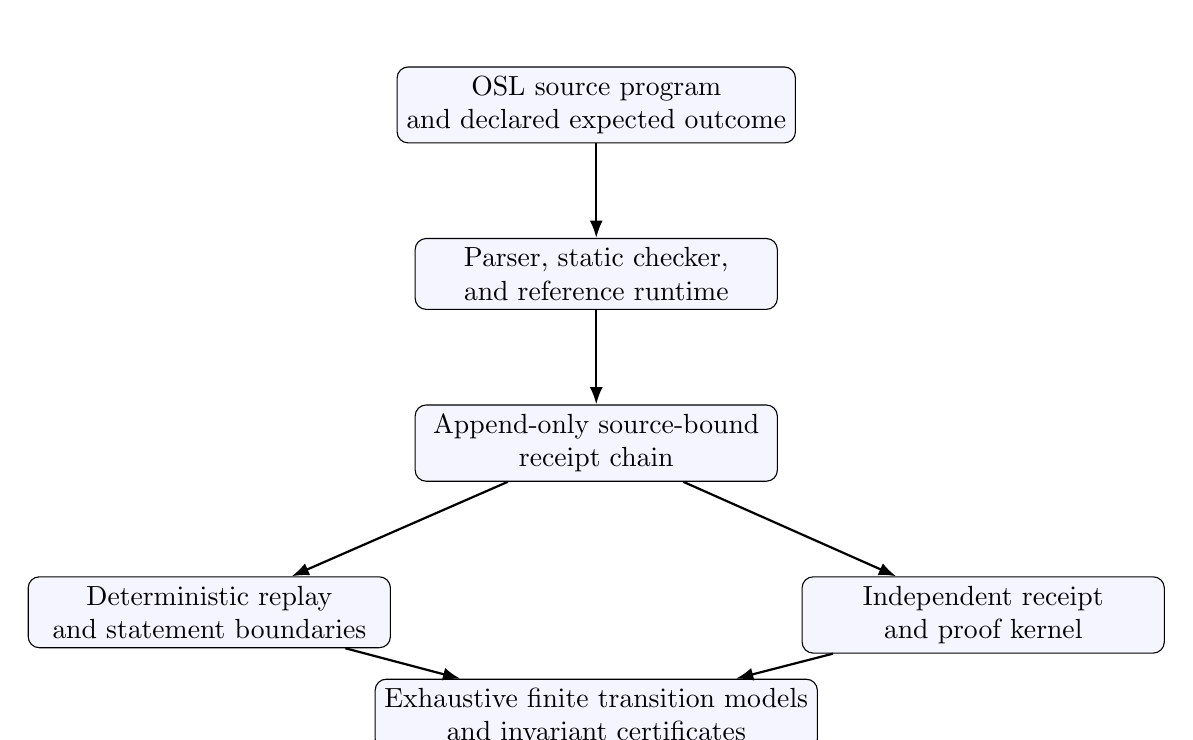
\begin{tikzpicture}[
  node distance=1.2cm,
  box/.style={draw,rounded corners,align=center,minimum width=4.6cm,minimum height=0.85cm,fill=blue!4},
  arr/.style={-{Latex[length=2.2mm]},thick}
]
\node[box] (src) {OSL source program\\and declared expected outcome};
\node[box,below=of src] (run) {Parser, static checker,\\and reference runtime};
\node[box,below=of run] (audit) {Append-only source-bound\\receipt chain};
\node[box,below left=1.2cm and 0.3cm of audit] (trace) {Deterministic replay\\and statement boundaries};
\node[box,below right=1.2cm and 0.3cm of audit] (kernel) {Independent receipt\\and proof kernel};
\node[box,below=2.5cm of audit] (finite) {Exhaustive finite transition models\\and invariant certificates};
\draw[arr] (src)--(run);
\draw[arr] (run)--(audit);
\draw[arr] (audit)--(trace);
\draw[arr] (audit)--(kernel);
\draw[arr] (trace)--(finite);
\draw[arr] (kernel)--(finite);
\end{tikzpicture}
\caption{The v0.3 trust stack.  The independent kernel reduces reliance on the runtime's self-description, while the finite abstractions check complete bounded state spaces rather than only source examples.}
\label{fig:v03-trust-stack}
\end{figure}

\begin{theorem}[Finite receipt-kernel soundness relative to its rules]
\label{thm:receipt-kernel-relative}
For a finite audit sequence accepted by the independent OSL-Core 0.3 kernel, every reconstructed observed-memory record has a source-consistent direct-observation token, every consumed affine or linear proof was previously constructed and available, every accepted execution is backed by an available capability, and every session advance follows a declared transition.
\end{theorem}

\begin{proof}
The verifier processes receipts in order.  Packet, proof, capability, action, and session tables are populated only through corresponding constructor receipts whose canonical digests are checked.  Each protected operation queries the reconstructed table before updating it.  Observed memory requires a compatible packet provenance and observation token; proof consumption requires availability; execution requires a reconstructed grant with positive unexpired capacity; and session advancement requires a matching transition tuple.  A violation records a failed kernel property and prevents acceptance.  The theorem is relative to this finite verifier and its declared receipt grammar.  \qedhere
\end{proof}

The packaged 66-program suite produced 1,149 audit receipts, 70 proof terms, 13 memory records, and two rollback events.  All 66 traces were independently accepted by the kernel, including the 24 programs whose intended result was safe rejection.

\subsection{Complete finite abstract kernel}

The integrated abstract kernel compresses packet, provenance, proof, capability, planning, and feedback status into a finite state tuple
\[
z=(\rho,a,b,q,e,u,m,c,p,x,f,\ldots).
\]
A finite alphabet of 26 commands includes observation, simulation, injection, admission, communication, binding, quarantine, endorsement, authorization, proof derivation, planning, capability grant or revocation, execution, feedback, and typed memory writes.

Let \(K_0\) be the initial state and \(\delta:K\times\Sigma\to K+\mathsf{Reject}\) the deterministic abstract transition.  Breadth-first exploration computes the least reachable fixpoint
\[
\mathsf{Reach}(K_0)
=
\mu X.\left(\{K_0\}\cup\delta(X,\Sigma)\right),
\]
where rejected transitions remain explicit outcomes but do not add new states.

\begin{theorem}[Exhaustive integrated-kernel certificate]
\label{thm:integrated-kernel-certificate}
For the declared OSL-Core 0.3 abstract kernel, exhaustive exploration reaches exactly 740 states and examines 19,240 state-command pairs.  All reachable states satisfy the declared well-formedness predicate, and every transition satisfies the finite checks for preservation, progress with explicit rejection, provenance non-forging, ownership gating, quarantine confinement, proof freshness, effect confinement, capability consumption, feedback causality, contract-obligation creation and discharge, and source preservation.
\end{theorem}

\begin{proof}
The certificate enumerates the finite state graph by breadth-first search until no new state is discovered.  For each reached state and every command in the fixed alphabet, it computes the transition, checks post-state well-formedness where accepted, and evaluates the declared transition properties.  The emitted graph digest commits to the sorted states, commands, and edges.  The packaged certificate reports zero failures.  This is a computer-assisted exhaustive proof for the encoded finite model.  \qedhere
\end{proof}

The certificate records 6,464 accepted and 12,776 explicitly rejected transitions.  Rejection is part of progress: a well-formed state and command either produce one well-formed successor or one declared finite error reason.

\subsection{Decomposed finite metacore}

A second metatheory implementation uses five smaller transition systems.  This decomposition makes model assumptions and checked invariants easier to inspect.  \Cref{tab:metacore-results} reports the complete fixpoints.

\begin{table}[ht]
\centering
\small
\begin{tabular}{@{}p{0.25\textwidth}rrp{0.39\textwidth}@{}}
\toprule
Model & States & Attempts & Principal check \\
\midrule
Provenance/ownership & 1,301 & 26,020 & no forged observed memory \\
Bounded capability & 256 & 2,560 & confinement and one-use consumption \\
Feedback deadline & 24 & 96 & no overdue accepted state \\
Transaction atomicity & 6 & 36 & rollback equivalence \\
Session fidelity & 3 & 6 & trace follows protocol \\
\midrule
Total & 1,590 & 28,718 & all declared checks pass \\
\bottomrule
\end{tabular}
\caption{Complete finite fixpoints in the decomposed metacore.  Accepted and rejected transition counts are retained in the machine-readable certificate.}
\label{tab:metacore-results}
\end{table}

\begin{theorem}[Decomposed finite preservation and safe progress]
For each model in \cref{tab:metacore-results}, every reachable state is well formed, every accepted transition preserves well-formedness and its model-specific invariant, and every attempted command either reaches one accepted successor or one explicit rejected outcome.  The listed state sets are fixed points of their respective reachability operators.
\end{theorem}

\begin{proof}
Each finite model supplies an initial state, command alphabet, well-formedness predicate, admissibility predicate, deterministic step function, and invariant family.  The common explorer performs complete breadth-first enumeration, evaluates every command from every reached state, and checks that the resulting discovered set is closed.  The five packaged certificates contain no counterexample and report fixed-point completion.  \qedhere
\end{proof}

Together, the integrated and decomposed models reach
\[
740+1{,}590=2{,}330
\]
abstract states and evaluate
\[
19{,}240+28{,}718=47{,}958
\]
finite transition cases.  These numbers must not be added to source-program counts as though they were independent empirical trials; they are complete checks of two formalized bounded abstractions.

\subsection{Verified finite session graphs}

The v0.2 session monitor enforced local message order.  Version 0.3 adds an offline graph verifier.  A finite protocol is
\[
\mathcal P=(Q,q_0,E,F),
\]
where \(Q\) is the finite state set, \(q_0\) the initial state, \(E\subseteq Q\times\mathsf{Msg}\times Q\) the transition relation, and \(F\subseteq Q\) the declared terminal states.

A protocol passes the finite verifier when:
\begin{enumerate}[label=(\roman*),leftmargin=1.7em]
  \item transition keys are deterministic;
  \item at least one terminal state is declared;
  \item every declared terminal is reachable;
  \item no reachable nonterminal state is a deadlock;
  \item no terminal state has an outgoing transition;
  \item every reachable state can reach a terminal state.
\end{enumerate}

\begin{theorem}[Finite protocol completion]
\label{thm:finite-protocol-completion}
If a finite protocol passes the conditions above, then every reachable nonterminal state has at least one finite path to a declared terminal, no accepted trace can advance after entering a terminal, and every monitored message step is a path in \(E\).
\end{theorem}

\begin{proof}
The final condition supplies a terminal-reaching path from every reachable state.  The deadlock condition excludes nonterminal states with no outgoing edge.  Terminal states have no outgoing transition, so the runtime deactivates the session upon entry and cannot accept a later monitored message.  Local runtime advancement checks membership in \(E\), establishing trace fidelity.  \qedhere
\end{proof}

\begin{lstlisting}[style=osl,caption={A finite protocol whose terminal state is verified before execution.}]
session CooperativeDiagnosis
    participants ["A","B"]
    initial waiting_A

session_transition CooperativeDiagnosis waiting_A
    communicate A B -> waiting_B
session_transition CooperativeDiagnosis waiting_B
    communicate B A -> ready
session_terminal CooperativeDiagnosis ready
verify_session CooperativeDiagnosis
start_session CooperativeDiagnosis
\end{lstlisting}

The packaged negative programs exhibit three distinct rejections: a reachable nonterminal deadlock, a terminal state with outgoing transitions, and an attempted start of a declared-terminal protocol that was not first verified.

\subsection{Static and dynamic information-flow certificates}

The restricted static information-flow fragment treats private secrets and public metadata as nodes in a dependency graph.  An explicit statement
\begin{lstlisting}[style=osl,numbers=none]
metadata covert from_secret private_goal source agent
\end{lstlisting}
adds an edge
\[
\mathsf{secret:private\_goal}\to\mathsf{metadata:covert}.
\]
A program passes the static certificate when no path exists from any declared secret to any declared public metadata node.

\begin{theorem}[Explicit-flow noninterference in the supported fragment]
For a program in the finite metadata fragment, if the static dependency graph has no path from a declared secret to a public metadata node, then changing secret values while holding all nonsecret literal metadata declarations fixed cannot change metadata values through the supported explicit \texttt{from\_secret} construction.
\end{theorem}

\begin{proof}
The only secret-dependent metadata constructor in the supported grammar introduces a direct dependency edge.  In its absence, public metadata values are functions only of their literal declarations.  Hence changing a secret cannot alter those values through a supported explicit dependency.  The statement does not cover implicit control flow, timing, operator choice, floating-point residues, or external tools.  \qedhere
\end{proof}

The static checker classifies both safe metadata examples as noninterfering and both deliberate leak examples as leaking.  A separate paired-run audit executes two programs that differ only in the secret.  The safe public projections are identical; the deliberate leak differs at both the public value and its digest.  The static and dynamic tests are complementary: one checks source dependency in a restricted grammar, while the other checks one declared pair of actual executions.

\subsection{Integrated verification totals}

\Cref{tab:v03-evidence} summarizes the packaged v0.3 evidence after regeneration from the same source tree.

\begin{table}[ht]
\centering
\begin{tabular}{lr}
\toprule
Evidence item & Verified count \\
\midrule
Source programs matching declared outcome & 66 of 66 \\
Accepted source programs & 42 \\
Expected safe rejections & 24 \\
Paired public-projection audits & 2 of 2 \\
Deterministically replayed source traces & 66 of 66 \\
Independently verified receipt traces & 66 of 66 \\
Independently reconstructed receipts & 1,149 \\
Independently reconstructed proof terms & 70 \\
Focused Python tests & 61 \\
Integrated abstract states & 740 \\
Integrated abstract transitions & 19,240 \\
Decomposed abstract states & 1,590 \\
Decomposed transition attempts & 28,718 \\
Total finite abstract states & 2,330 \\
Total finite transition checks & 47,958 \\
\bottomrule
\end{tabular}
\caption{Finite OSL-Core 0.3 verification evidence.  Counts refer to different evidence layers and are not interchangeable empirical sample sizes.}
\label{tab:v03-evidence}
\end{table}

The source suite includes positive examples for exactly-once proof consumption, affine nonuse, terminal session verification, explicit receipt-chain checking, linear ownership proofs, and a three-agent verified protocol.  Negative cases cover proof reuse, unmet linear obligations, reachable protocol deadlock, terminal outgoing edges, unverified session start, and reuse of a consumed linear ownership proof.

\begin{provedbox}
Within the declared finite semantics, OSL-Core 0.3 now has executable evidence for: source-level conformance; deterministic semantic replay; statement-boundary continuity; append-only rollback auditing; persistent, affine, and linear proof resources; independent proof and receipt reconstruction; provenance non-forging; capability confinement; feedback obligations; finite session safety and terminal reachability; and explicit secret-to-metadata flow detection.
\end{provedbox}

\subsection{What the computer-assisted results do and do not prove}

The finite results strengthen the project in three ways.  First, they remove dependence on a handful of illustrative programs by checking complete abstract state spaces.  Second, they reduce circular trust by reconstructing semantic objects from receipts with a separately written kernel.  Third, they make negative behavior first class: safe rejection, rollback, proof exhaustion, contract violation, and protocol deadlock are represented and verified rather than treated as incidental exceptions.

They do not establish that the full interpreter is free of implementation bugs.  Both Python implementations may share a misunderstood specification.  Cryptographic receipts provide tamper evidence, not principal authentication.  Trusted neural attestations remain trust roots.  The static flow certificate covers an explicit syntax fragment rather than arbitrary covert channels.  Session verification is finite and synchronous rather than a proof of general asynchronous multiparty liveness.

\begin{placeholderbox}
\textbf{Proof-assistant correspondence.}  The next metatheoretic milestone is a small mechanized calculus whose syntax, typing, operational semantics, proof-resource accounting, and receipt relation are defined in a proof assistant.  The primary targets are preservation, progress with declared rejection, linear-resource conservation, receipt-to-transition correspondence, rollback equivalence, and extraction of a verified checker.  The current exhaustive certificates provide executable specifications and regression oracles for that development; they are not a substitute for it.
\end{placeholderbox}

\subsection{Reproducible verification pipeline}

The packaged pipeline is:
\begin{verbatim}
source examples
  -> parser and static checker
  -> deterministic source execution
  -> append-only audit traces
  -> deterministic replay verifier
  -> independent receipt/proof kernel
  -> integrated finite kernel
  -> decomposed finite metacore
  -> unified certificate
\end{verbatim}
The unified certificate commits to the component certificate digests and records the finite claim boundary.  Rebuilding a component changes the unified verification digest.  This produces a compact, auditable map from source examples to the finite abstract theorems stated in this section.


\section{Denotational semantics}

\subsection{Types and terms}

A denotational model \(\mathfrak M\) assigns:
\[
\Sem{\tau}_{\mathfrak M}=X_\tau
\]
to each type and
\[
\Sem{g}_{\mathfrak M}:X_\tau\to X_\sigma
\]
to each typed operator \(g:\tau\to\sigma\).

\subsection{Formula semantics}

For a crisp finite model, each formula denotes a subset of system states:
\[
\Sem{\varphi}_{\mathfrak M}\subseteq\mathcal S.
\]
For probabilistic or four-valued models, the codomain is generalized later.

\subsection{Graded semantics}

For approximate models, a formula may denote a score
\[
v_{\mathfrak M}(\varphi,s)\in[0,1]
\]
or a support--refutation pair in \([0,1]^2\). A threshold \(\theta\) creates a derived crisp judgment, but the unthresholded score is retained for calibration and stability analysis. The language therefore separates
\[
\text{semantic score},\qquad
\text{decision threshold},\qquad
\text{authorization policy}.
\]
A high semantic score alone does not authorize an irreversible action.

\subsection{Dynamic semantics}

\[
s\models[\alpha]\varphi
\]
iff every \(s'\) with \((s,s')\in\Sem{\alpha}\) satisfies \(s'\models\varphi\).

\subsection{Causal semantics}

An operator symbol is not fully grounded merely because it has a denotation. It is behaviorally grounded when intervention on its represented state produces the predicted family of consequences. For an operator \(g\) and causal outcome map \(Y\), define the grounding residual
\[
\epsilon_{\mathrm{causal}}(g)
=
\mathbb E_{x,\delta}
\left[
\left\|
Y(g(x+\delta))-Y(g(x))-D(Y\circ g)_x\delta
\right\|
\right].
\]
Small residual supports a local first-order causal interpretation; it does not establish universal correctness.

\subsection{Coalgebraic trace semantics}

For a finite action alphabet \(\mathsf A\), a deterministic agent can be represented by an observation map \(o:S\to O\) and transitions
\[
\delta_a:S\to S,
\qquad a\in\mathsf A.
\]
Equivalently,
\[
\gamma:S\to O\times S^{\mathsf A},
\qquad
\gamma(s)=\left(o(s),(\delta_a(s))_{a\in\mathsf A}\right).
\]

\begin{definition}[Coalgebra homomorphism]
A map \(T:S_A\to S_B\) is a coalgebra homomorphism when
\[
o_B(Ts)=o_A(s)
\]
and
\[
T\delta^A_a(s)=\delta^B_a(Ts)
\]
for every state and action.
\end{definition}

\begin{theorem}[Finite-trace preservation]
A coalgebra homomorphism preserves every finite action-conditioned observation trace. For each word
\[
w=a_n\cdots a_1,
\]
the two systems produce identical observation sequences from \(s\) and \(T(s)\).
\end{theorem}

\begin{proof}
The initial observations agree by definition. The transition equation carries corresponding states to corresponding states after one action. Induction over word length preserves every later observation.
\end{proof}

\begin{figure}[ht]
\centering
\begin{tikzcd}[column sep=large,row sep=large]
S_A \arrow[r,"\gamma_A"] \arrow[d,"T"'] & O\times S_A^{\mathsf A} \arrow[d,"I_O\times T^{\mathsf A}"] \\
S_B \arrow[r,"\gamma_B"'] & O\times S_B^{\mathsf A}
\end{tikzcd}
\caption{Coalgebraic semantic transport. Commutation preserves action-conditioned behavior, not merely static representations.}
\label{fig:coalgebra}
\end{figure}

This result complements algebraic intertwining. The algebra view preserves compositional transformations; the coalgebra view preserves observable behavior through time.

\section{Meaning as shared algebra rather than shared coordinates}

\subsection{Heterogeneous internal spaces}

Let agents \(A\) and \(B\) possess latent spaces \(\Lat_A\) and \(\Lat_B\). Both realize an abstract algebra \(\mathcal A\):
\[
\rho_A:\mathcal A\to\End(\Lat_A),
\qquad
\rho_B:\mathcal A\to\End(\Lat_B).
\]
A map
\[
T_{A\to B}:\Lat_A\to\Lat_B
\]
preserves operator meaning when
\begin{equation}
T_{A\to B}\rho_A(g)
=
\rho_B(g)T_{A\to B}.
\label{eq:intertwiner}
\end{equation}
for all relevant \(g\in\mathcal A\).

\begin{definition}[Exact semantic intertwiner]
A linear map \(T:\Lat_A\to\Lat_B\) satisfying \cref{eq:intertwiner} for all \(g\in\mathcal A\) is an exact semantic intertwiner between the two realizations.
\end{definition}

\begin{theorem}[Preservation of algebraic semantics]
Let \(T:\Lat_A\to\Lat_B\) be an exact semantic intertwiner. For every noncommutative polynomial \(p\) in generators of \(\mathcal A\),
\[
T\,p(\rho_A(g_1),\ldots,\rho_A(g_m))
=
p(\rho_B(g_1),\ldots,\rho_B(g_m))\,T.
\]
\end{theorem}

\begin{proof}
The result holds for generators by assumption and for the identity trivially. It is preserved under addition and scalar multiplication by linearity. If it holds for words \(u\) and \(v\), then
\[
T\rho_A(uv)
=T\rho_A(u)\rho_A(v)
=\rho_B(u)T\rho_A(v)
=\rho_B(u)\rho_B(v)T
=\rho_B(uv)T.
\]
Induction over word length and linear extension yield the polynomial statement.
\end{proof}

\begin{corollary}[Compositional transfer]
If two agents share an exact intertwiner for the primitive operator algebra, then every finite symbolic program built by operator composition is transported consistently.
\end{corollary}

\subsection{Approximate intertwiners}

For noisy systems define
\[
\epsilon_T(g)
=
\left\|
T\rho_A(g)-\rho_B(g)T
\right\|.
\]

\begin{proposition}[Product error bound]
For operators \(g_1,\ldots,g_n\),
\[
\begin{aligned}
&\left\|
T\rho_A(g_n\cdots g_1)
-
\rho_B(g_n\cdots g_1)T
\right\|\\
&\qquad\le
\sum_{k=1}^{n}
\left(
\prod_{j=k+1}^{n}\|\rho_B(g_j)\|
\right)
\epsilon_T(g_k)
\left(
\prod_{j=1}^{k-1}\|\rho_A(g_j)\|
\right).
\end{aligned}
\]
\end{proposition}

\begin{proof}
Insert and subtract intermediate terms that move \(T\) across one factor at a time, then apply the triangle inequality and submultiplicativity.
\end{proof}

\begin{corollary}[Approximate preservation of presented relations]
Assume every generator realization has norm at most \(M\) and
\[
\epsilon_T(g)\le\epsilon
\]
for each generator. Let
\[
p=\sum_w c_w w
\]
be a finite noncommutative polynomial relation, where \(|w|\) is word length. If \(p(\rho_A)=0\), then
\[
\left\|p(\rho_B)T\right\|
\le
\epsilon
\sum_w
|c_w|\,|w|\,M^{|w|-1}.
\]
\end{corollary}

\begin{proof}
Apply the product error bound to every word and use
\[
Tp(\rho_A)-p(\rho_B)T=-p(\rho_B)T.
\]
Linearity and the triangle inequality give the result.
\end{proof}

\subsection{Gauge equivalence}

Let \(S:\Lat_A\to\Lat_A\) be invertible. Define
\[
z'=Sz,
\qquad
\rho_A'(g)=S\rho_A(g)S^{-1}.
\]

\begin{theorem}[Gauge invariance of operator meaning]
The representations \(\rho_A\) and \(\rho_A'\) satisfy the same algebraic identities. In particular, if
\[
p(\rho_A(g_1),\ldots,\rho_A(g_m))=0,
\]
then
\[
p(\rho_A'(g_1),\ldots,\rho_A'(g_m))=0.
\]
\end{theorem}

\begin{proof}
Every polynomial expression transforms by conjugation:
\[
p(\rho_A'(g_1),\ldots,\rho_A'(g_m))
=
S\,p(\rho_A(g_1),\ldots,\rho_A(g_m))\,S^{-1}.
\]
The conclusion follows.
\end{proof}

\begin{remark}
External interaction may constrain an internal algebra up to gauge without fixing one neuron, coordinate, basis, or embedding direction. The invariant object is the relation among transformations.
\end{remark}

\begin{figure}[ht]
\centering
\begin{tikzcd}[column sep=large,row sep=large]
\Lat_A \arrow[r,"\rho_A(g)"] \arrow[d,"T_{A\to B}"'] & \Lat_A \arrow[d,"T_{A\to B}"] \\
\Lat_B \arrow[r,"\rho_B(g)"'] & \Lat_B
\end{tikzcd}
\caption{Meaning preservation as an intertwining relation. The diagram commutes exactly or approximately even when the two agents use different coordinates.}
\label{fig:intertwiner}
\end{figure}

\section{Symbols as compressed operator invariants}

\subsection{Functional equivalence}

Let \(\mathcal O\) be a set of concrete operations. Define an equivalence relation
\[
\alpha\sim\beta
\]
when \(\alpha\) and \(\beta\) are indistinguishable under all declared tests, contexts, and relevant consequences.

\begin{definition}[Operator congruence]
An equivalence relation \(\sim\) on \(\mathcal O\) is a congruence if
\[
\alpha\sim\beta
\quad\Longrightarrow\quad
\gamma\circ\alpha\circ\delta
\sim
\gamma\circ\beta\circ\delta
\]
whenever the compositions are well typed.
\end{definition}

\begin{theorem}[Quotient symbol algebra]
If \(\sim\) is an operator congruence, then composition on equivalence classes
\[
[\alpha]\cdot[\beta]
:=
[\alpha\circ\beta]
\]
is well defined. The quotient \(\mathcal O/{\sim}\) forms a typed operator algebra whenever \(\mathcal O\) does.
\end{theorem}

\begin{proof}
If \(\alpha\sim\alpha'\) and \(\beta\sim\beta'\), congruence gives
\[
\alpha\circ\beta
\sim
\alpha'\circ\beta
\sim
\alpha'\circ\beta'.
\]
Thus the product does not depend on representatives. All inherited algebraic laws descend to the quotient.
\end{proof}

\begin{remark}
A symbol can therefore be interpreted as a name for a stable equivalence class of operations or relations, rather than an arbitrary token assigned before learning.
\end{remark}

\subsection{Developmental sequence}

The proposed emergence path is:
\[
\begin{aligned}
\text{repeated interaction}
&\to
\text{recurring operator pattern}
\to
\text{functional equivalence class}\\
&\to
\text{compressed symbol}
\to
\text{symbolic composition}.
\end{aligned}
\]

\begin{conjecture}[Interaction-algebra internalization]
Suppose an agent is trained on a family of tasks generated by an algebra \(\mathcal A\), with losses that reward compositional generalization and penalize representation complexity. Under suitable identifiability and optimization assumptions, the learned latent dynamics converge, up to gauge and approximation error, to a representation of a quotient of \(\mathcal A\).
\end{conjecture}

\subsection{Finite observational recovery}

Let \(\mathfrak C=\{C_1,\ldots,C_m\}\) be a finite family of well-typed one-hole contexts and let
\[
\operatorname{Out}(C_i[\alpha])
\]
be the declared observable consequence of placing operation \(\alpha\) in context \(C_i\).

\begin{definition}[Observational signature]
The finite signature of \(\alpha\) is
\[
\Sig_{\mathfrak C}(\alpha)
=
\left(
\operatorname{Out}(C_1[\alpha]),\ldots,
\operatorname{Out}(C_m[\alpha])
\right).
\]
Define \(\alpha\sim_{\mathfrak C}\beta\) iff their signatures agree.
\end{definition}

\begin{theorem}[Finite contextual congruence]
The relation \(\sim_{\mathfrak C}\) is an equivalence relation. If \(\mathfrak C\) is closed under every well-typed left and right composition by primitive operations, then \(\sim_{\mathfrak C}\) is an operator congruence.
\end{theorem}

\begin{proof}
Equality of signatures is reflexive, symmetric, and transitive. For congruence, suppose \(\alpha\sim_{\mathfrak C}\beta\). For compatible primitives \(\gamma,\delta\) and any test context \(D\), define
\[
C[\cdot]=D[\gamma\circ(\cdot)\circ\delta].
\]
Closure gives \(C\in\mathfrak C\), so equality of \(\alpha\) and \(\beta\) under \(C\) implies equality of \(\gamma\circ\alpha\circ\delta\) and \(\gamma\circ\beta\circ\delta\) under \(D\).
\end{proof}

\begin{algorithm}[ht]
\caption{Finite observational symbol discovery}
\label{alg:symbol-discovery}
\begin{algorithmic}[1]
\Require finite typed operation set \(\mathcal O\), context suite \(\mathfrak C\)
\ForAll{\(\alpha\in\mathcal O\)}
  \State evaluate \(\Sig_{\mathfrak C}(\alpha)\)
\EndFor
\State partition \(\mathcal O\) by equality of signatures
\State return quotient classes and the induced composition table
\end{algorithmic}
\end{algorithm}

\begin{proposition}[Relative soundness and completeness]
Algorithm~\ref{alg:symbol-discovery} returns exactly the equivalence classes of \(\sim_{\mathfrak C}\). Under contextual closure, its composition table is well defined.
\end{proposition}

\begin{proof}
Two operations are placed in the same block exactly when their signatures agree. The preceding theorem supplies well-defined quotient composition.
\end{proof}

\begin{remark}
With noisy outputs, an \(\epsilon\)-threshold relation need not be transitive. Practical discovery should therefore use confidence regions, complete-linkage constraints, or explicit congruence closure rather than naive pairwise thresholding.
\end{remark}

\begin{placeholderbox}
The finite result is relative to a declared context suite. Discovering a minimal task-sufficient congruence under distribution shift, continuous operation families, and adaptive adversarial contexts remains open. The conjecture above is therefore narrowed, not proved in full.
\end{placeholderbox}

\section{Logical structure realized geometrically}

\subsection{Candidate geometries}

Logical structure may be represented by geometry rather than explicit rule tables.

\begin{center}
\begin{tabular}{ll}
\toprule
Logical relation & Candidate geometric realization \\
\midrule
Equivalence & clusters or quotient spaces \\
Negation & involution \(N^2\approx I\) \\
Implication & order cone \\
Conjunction & tensor or bilinear product \\
Temporal succession & semigroup flow \\
Reversible transformation & group action \\
Hierarchy & tree or hyperbolic geometry \\
Provenance & fiber indexed by source lineage \\
Fork & branching cospan \\
Shared meaning & common quotient or interlingua \\
\bottomrule
\end{tabular}
\end{center}

\subsection{Implication cones}

Let \(C\subseteq\Lat\) be a closed convex cone. One candidate semantics is
\[
p\Rightarrow q
\quad\Longleftrightarrow\quad
z_q-z_p\in C.
\]
This gives implication a partial-order geometry when \(C\cap(-C)=\{0\}\).

\subsection{Negation}

A negation operator may satisfy
\[
N^2=I.
\]
If propositions are represented as regions or subspaces, \(N\) should exchange a proposition with an appropriately defined contradictory region rather than merely multiply every vector by \(-1\).

\subsection{Conjunction}

A higher-order conjunction may use a typed bilinear map
\[
\mu_{\wedge}:\Lat_\varphi\otimes\Lat_\psi\to\Lat_{\varphi\wedge\psi}.
\]
The tensor product records that conjunction may depend on interactions not reducible to a sum of independent features.

\subsection{A finite ordered geometric fragment}

\begin{definition}[Order cone]
Let \(V\) be a real vector space and \(C\subseteq V\) a convex cone. Define
\[
x\preceq_C y
\quad\Longleftrightarrow\quad
y-x\in C.
\]
The cone is \emph{pointed} when \(C\cap(-C)=\{0\}\).
\end{definition}

\begin{proposition}[Cone order]
If \(C\) is a pointed convex cone, then \(\preceq_C\) is a partial order.
\end{proposition}

\begin{proof}
Reflexivity follows from \(0\in C\), transitivity from closure under addition, and antisymmetry from pointedness.
\end{proof}

\begin{theorem}[Ordered involutive operator fragment]
Let \(C\subseteq V\) be a pointed convex cone. Suppose \(N:V\to V\) is linear with
\[
N^2=I,
\qquad
N(C)=-C,
\]
and \(\mu:V\otimes V\to V\) is bilinear, associative, commutative, has unit \(e\), and is positive in the sense that
\[
\mu(C,C)\subseteq C.
\]
Then \((V,\preceq_C,\mu,e,N)\) is an ordered involutive commutative monoid: \(N\) reverses the order and \(\mu\) is monotone in each argument on \(C\).
\end{theorem}

\begin{proof}
The cone proposition gives the order. If \(x\preceq_C y\), then \(y-x\in C\), so
\[
N(x)-N(y)=-N(y-x)\in C,
\]
hence \(N(y)\preceq_C N(x)\). Positivity and bilinearity imply
\[
\mu(y,z)-\mu(x,z)=\mu(y-x,z)\in C
\]
for \(z\in C\), and similarly in the second argument. The monoid laws are assumed.
\end{proof}

\begin{remark}
This theorem realizes a useful logical fragment geometrically, but it does not imply Boolean idempotence, excluded middle, complement laws, or distributivity. Those laws must be declared separately and tested against the intended probabilistic, paraconsistent, or resource-sensitive semantics.
\end{remark}

\section{Probabilistic and paraconsistent semantics}

\subsection{Four-valued support}

For a proposition \(p\), store
\[
v(p)=(s(p),r(p))\in[0,1]^2,
\]
where \(s\) is support and \(r\) is refutation.

\begin{center}
\begin{tabular}{lll}
\toprule
Region & Interpretation & Default policy \\
\midrule
high \(s\), low \(r\) & provisionally accepted & permit authorized use \\
low \(s\), high \(r\) & provisionally rejected & do not use \\
high \(s\), high \(r\) & conflicted & quarantine \\
low \(s\), low \(r\) & unresolved & seek evidence or abstain \\
\bottomrule
\end{tabular}
\end{center}

\subsection{No explosion}

The logic should not validate
\[
p,\neg p\vdash q
\]
for arbitrary \(q\). Conflicting autobiographical or communicated content must remain localized.

A concrete four-valued algebra uses
\[
\neg(s,r)=(r,s),
\]
\[
(s_1,r_1)\wedge(s_2,r_2)
=
(\min\{s_1,s_2\},\max\{r_1,r_2\}),
\]
\[
(s_1,r_1)\vee(s_2,r_2)
=
(\max\{s_1,s_2\},\min\{r_1,r_2\}).
\]
A contradiction changes the value of formulas that actually depend on it; it does not assign arbitrary values to unrelated propositions.

\subsection{Quantitative semantic stability}

Let \(\Theta\) denote the tuple of operator interpretations and let \(d(\Theta,\Theta')\) measure representation error. Assume atomic valuations are Lipschitz, the selected connectives are nonexpansive under the sup metric, and every modal interpretation \(M\) is \(L_M\)-Lipschitz.

\begin{theorem}[Structural stability of graded formulas]
For every formula \(\varphi\) there exists a recursively computable constant \(L_\varphi\) such that
\[
\left|
 v_\Theta(\varphi,s)-v_{\Theta'}(\varphi,s)
\right|
\le
L_\varphi\,d(\Theta,\Theta').
\]
One may take
\[
L_{\neg\varphi}=L_\varphi,
\qquad
L_{\varphi\wedge\psi}=\max\{L_\varphi,L_\psi\},
\qquad
L_{M\varphi}=L_ML_\varphi,
\]
with analogous rules for the remaining nonexpansive connectives.
\end{theorem}

\begin{proof}
Proceed by structural induction. The atomic case is the Lipschitz assumption. Nonexpansiveness proves the connective steps. The modal step follows by composing Lipschitz maps.
\end{proof}

\begin{corollary}[Threshold robustness]
If a decision threshold \(\theta\) has margin
\[
\left|v_\Theta(\varphi,s)-\theta\right|
>
L_\varphi d(\Theta,\Theta'),
\]
then the thresholded decision is unchanged under replacement of \(\Theta\) by \(\Theta'\).
\end{corollary}

\subsection{Confidence as a first-class term}

Endorsement may be represented by
\[
K_a^q\varphi,
\qquad q\in[0,1].
\]
The confidence value should be calibrated against observed success and tied to a declared evidence context.

\subsection{Decision rules}

A risk-sensitive action rule may require
\[
J_a\varphi
\wedge
K_a^q\varphi
\wedge
q\ge\theta
\wedge
\Auth_a(\varphi)
\to
U_a\varphi.
\]
The threshold \(\theta\) depends on action cost and reversibility.

\section{Provenance and proof-carrying execution}

\subsection{Provenance records}

A content packet is
\[
e=(c,a_{\mathrm{src}},L_{\mathrm{src}},\kappa,t,q,\mathcal A,d),
\]
where \(c\) is content, \(a_{\mathrm{src}}\) source agent, \(L_{\mathrm{src}}\) source lineage, \(\kappa\) origin type, \(t\) time, \(q\) confidence, \(\mathcal A\) permitted uses, and \(d\) an integrity digest.

\subsection{Content is not ownership}

\begin{theorem}[Content-only ownership impossibility]
Let two events \(e_1,e_2\) have identical accessible content \(C(e_1)=C(e_2)=c\), but opposite ownership labels. No classifier \(f(c)\) depending only on content can classify both correctly.
\end{theorem}

\begin{proof}
Because the input is identical, \(f(C(e_1))=f(c)=f(C(e_2))\), while the correct outputs differ.
\end{proof}

\begin{corollary}[Equiprobable ownership lower bound]
If the two provenance cases are equiprobable, every content-only classifier has error at least \(1/2\) on the pair.
\end{corollary}

\subsection{Proof-gated actions}

Let \(\operatorname{Pre}(\alpha)\) denote the logical precondition of action \(\alpha\). An executor accepts \((\alpha,p)\) only when the verifier establishes
\[
p:\operatorname{Pre}(\alpha).
\]

\begin{assumption}[Verifier soundness]
Whenever the verifier accepts \(p:\varphi\), the proposition \(\varphi\) is true in the current operational model.
\end{assumption}

\begin{theorem}[Proof-gated execution safety]
Under verifier soundness, every executed action \(\alpha\) satisfies its declared precondition \(\operatorname{Pre}(\alpha)\).
\end{theorem}

\begin{proof}
The executor runs \(\alpha\) only after acceptance of a proof term \(p:\operatorname{Pre}(\alpha)\). Soundness implies the precondition holds at execution time.
\end{proof}

\begin{remark}
A cryptographic digest proves byte integrity, not semantic authorization. The verifier must check lineage, provenance, conflict status, and action-specific constraints.
\end{remark}

\subsection{Linear provenance resources}

A direct observation token \(\Obs_A(c)\) should not be freely duplicable across agents. Communication may use the rule
\[
\Obs_A(c)
\multimap
\bigl(
\Access_B(c)
\otimes
\Origin_A(c)
\bigr),
\]
not
\[
\Obs_A(c)\multimap\Obs_B(c).
\]
This preserves the distinction between access and personal observation.

\subsection{Proof transport between calculi}

Let \(\mathcal L_A\) and \(\mathcal L_B\) be typed proof calculi. A translation \(\Theta\) maps source types, formulas, contexts, and proof constructors into the target calculus.

\begin{theorem}[Syntactic proof transport]
Assume:
\begin{enumerate}[leftmargin=1.7em]
  \item every source axiom \(\varphi\) maps to a target theorem \(\Theta(\varphi)\);
  \item for every source inference rule, the translated conclusion is derivable from the translated premises in the target calculus;
  \item translation preserves typing and linear-resource usage.
\end{enumerate}
Then
\[
\Gamma;\Pi\vdash_A\varphi
\quad\Longrightarrow\quad
\Theta(\Gamma);\Theta(\Pi)\vdash_B\Theta(\varphi).
\]
\end{theorem}

\begin{proof}
Induct on the source derivation. Axioms are covered by the first assumption. Each inference step transports by the second assumption, while the third preserves well-formedness and resource accounting.
\end{proof}

\begin{remark}
This theorem transports derivability, not trust. Agent B must still trust the translation, the target verifier, and any external evidence referenced by the proof. Approximate neural proof objects require an additional certificate or re-verification layer.
\end{remark}

\section{Shared operator-symbolic languages}

\subsection{Common interlingua}

Let \(\Shared\) be a shared operator-symbolic space. Agent encoders and decoders are
\[
E_A:\Lat_A\to\Shared,
\qquad
D_A:\Shared\to\Lat_A.
\]
Cross-agent transport is
\[
T_{A\to B}=D_BE_A.
\]

\subsection{Shared packet}

A shared packet is
\[
p=(c,o,L,\kappa,q,\mathcal A,t_{\mathrm{exp}},d).
\]
It contains content, origin, source lineage, provenance class, confidence, permitted uses, expiration, and digest.

\subsection{Functional transport objective}

A transport map should minimize
\[
\begin{aligned}
\mathcal L={}&
\lambda_1\mathcal L_{\mathrm{task}}
+\lambda_2\mathcal L_{\mathrm{recon}}
+\lambda_3\mathcal L_{\mathrm{func}}\\
&+\lambda_4\mathcal L_{\mathrm{cycle}}
+\lambda_5\mathcal L_{\mathrm{causal}}
+\lambda_6\mathcal L_{\mathrm{prov}}
+\lambda_7\mathcal L_{\mathrm{capacity}}.
\end{aligned}
\]

\subsection{Interlingua factorization}

\begin{proposition}[Exact shared factorization]
Suppose \(E_A:\Lat_A\to\Shared\) and \(D_B:\Shared\to\Lat_B\) satisfy
\[
E_A\rho_A(g)=\rho_\star(g)E_A,
\qquad
D_B\rho_\star(g)=\rho_B(g)D_B.
\]
Then \(T_{A\to B}=D_BE_A\) is an intertwiner:
\[
T_{A\to B}\rho_A(g)=\rho_B(g)T_{A\to B}.
\]
\end{proposition}

\begin{proof}
\[
D_BE_A\rho_A(g)
=D_B\rho_\star(g)E_A
=\rho_B(g)D_BE_A.
\]
\end{proof}

\begin{figure}[ht]
\centering
\resizebox{\textwidth}{!}{%
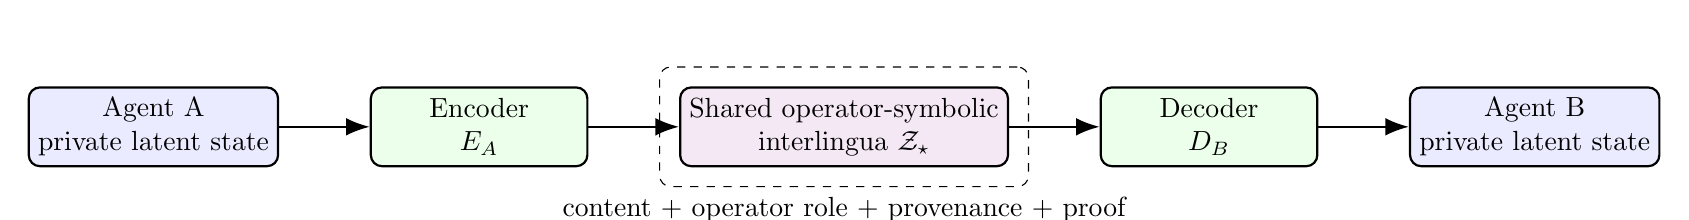
\begin{tikzpicture}[
  box/.style={draw,rounded corners,minimum width=2.75cm,minimum height=1cm,align=center,thick},
  arr/.style={-{Latex[length=3mm]},thick},
  node distance=1.0cm and 1.15cm
]
\node[box,fill=blue!8] (A) {Agent A\\private latent state};
\node[box,fill=green!8,right=of A] (EA) {Encoder\\\(E_A\)};
\node[box,fill=violet!9,right=of EA] (S) {Shared operator-symbolic\\interlingua \(\Shared\)};
\node[box,fill=green!8,right=of S] (DB) {Decoder\\\(D_B\)};
\node[box,fill=blue!8,right=of DB] (B) {Agent B\\private latent state};
\draw[arr] (A)--(EA);
\draw[arr] (EA)--(S);
\draw[arr] (S)--(DB);
\draw[arr] (DB)--(B);
\node[draw,dashed,rounded corners,fit=(S),inner sep=7pt,label=below:{content + operator role + provenance + proof}] {};
\end{tikzpicture}%
}
\caption{Heterogeneous agents communicate through a shared algebraic interlingua rather than by copying raw hidden states.}
\label{fig:shared}
\end{figure}

\subsection{Communication is not merger}

The agents remain distinct when private states, lineages, and independent control loops remain causally meaningful. A shared interlingua becomes a candidate group-level cognitive substrate only when critical state and recurrence exist irreducibly in the shared space.

\subsection{Interface-decomposable communication}

Let the joint deterministic state be \((x_A,x_B,w)\in X_A\times X_B\times W\). The system is \emph{interface decomposable} when
\[
\begin{aligned}
x_A'&=F_A(x_A,w),\\
x_B'&=F_B(x_B,w),\\
w'&=G(w,m_A(x_A),m_B(x_B)),
\end{aligned}
\]
so each agent depends on the other only through the declared shared interface.

\begin{theorem}[Private closure under a channel cut]
Let \(C_A\subseteq X_A\) and \(C_B\subseteq X_B\) be private invariant sets. Suppose a channel cut replaces \(w\) by a fixed safe value \(w_0\), and
\[
F_A(C_A,w_0)\subseteq C_A,
\qquad
F_B(C_B,w_0)\subseteq C_B.
\]
Then after the cut, each private system remains in its own invariant set for every future step.
\end{theorem}

\begin{proof}
Apply the two inclusion assumptions inductively over time.
\end{proof}

This supplies a sufficient operational criterion for communication between persistent agents: the shared interface may improve performance, but removing it does not destroy each private invariant process.

\subsection{Group-level task irreducibility}

Let \(Y\) be a task variable. If
\[
H(Y\mid X_A)>0,
\qquad
H(Y\mid X_B)>0,
\qquad
H(Y\mid X_A,X_B,W)=0,
\]
then neither private state alone determines the correct task output, while the joint state does.

\begin{theorem}[Necessity of a joint representation]
Under the entropy conditions above, no deterministic policy using only \(X_A\) or only \(X_B\) can solve every instance perfectly. A joint policy using \((X_A,X_B,W)\) can in principle do so.
\end{theorem}

\begin{proof}
Positive conditional entropy means at least two task outcomes remain possible after conditioning on the private state, so no deterministic private policy is always correct. Zero joint conditional entropy means \(Y\) is a function of the joint state.
\end{proof}

\begin{proposition}[Task-conditioned communication lower bound]
Let \(Y\) take values in a finite set \(\mathcal Y\), let \(X_B\) be Agent B's private state, and let \(M\) be a message used to estimate \(Y\) with error probability \(P_e\). Then
\[
I(Y;M\mid X_B)
\ge
H(Y\mid X_B)
-
 h_2(P_e)
-
P_e\log_2(|\mathcal Y|-1),
\]
where \(h_2\) is binary entropy.
\end{proposition}

\begin{proof}
By conditional Fano inequality,
\[
H(Y\mid M,X_B)
\le
h_2(P_e)+P_e\log_2(|\mathcal Y|-1).
\]
Subtract this bound from
\[
I(Y;M\mid X_B)=H(Y\mid X_B)-H(Y\mid M,X_B).
\]
\end{proof}

The bound is representation independent. Any text, vector, packet, or operator-symbolic channel achieving the same error must transmit the required conditional task information. The open problem is to characterize the additional rate needed to preserve operator relations, provenance, and proof obligations simultaneously.

\begin{placeholderbox}
The results separate private persistence from group-level task irreducibility, but they do not provide a necessary-and-sufficient criterion for cognitive merger. A complete criterion likely requires recurrent group closure, interventionally irreducible state, lineage policy, and a declared level of analysis.
\end{placeholderbox}

\subsection{Canonical metadata and covert capacity}

Let \(C\) be declared content, \(S\) prohibited private information, and \(M\) public metadata.

\begin{theorem}[Canonical metadata noninterference]
If trusted infrastructure computes metadata deterministically as
\[
M=g(C),
\]
then
\[
I(S;M\mid C)=0.
\]
\end{theorem}

\begin{proof}
Conditioned on \(C\), the value of \(M\) is fixed and therefore independent of \(S\).
\end{proof}

\begin{proposition}[Finite metadata capacity]
If, for each declared content value \(c\), metadata belongs to a finite admissible set \(\mathcal M_c\), then
\[
I(S;M\mid C=c)
\le
H(M\mid C=c)
\le
\log_2|\mathcal M_c|.
\]
For a sequence of \(n\) packets, capacity is at most the sum of the per-packet logarithmic bounds.
\end{proposition}

This does not prove the semantic channel is safe: agents may encode information in the declared operator choice itself. It does show why canonicalization, fixed precision, trusted timestamps, and finite codebooks remove whole classes of metadata channels.

\section{Komorebi-style operator grammar}

\subsection{Analysis, packets, transfer, synthesis}

A generic operator expression has the form
\[
x
\xrightarrow{\mathcal A}
(P_\alpha x)_\alpha
\xrightarrow{T_{\beta\alpha}}
(P_\beta T P_\alpha x)_{\beta,\alpha}
\xrightarrow{\mathcal S}
x'.
\]
The stages are:
\begin{enumerate}[leftmargin=1.7em]
  \item analyze a state into packets;
  \item select causally or semantically relevant packets;
  \item transport packet relations;
  \item validate provenance and residuals;
  \item synthesize an updated state.
\end{enumerate}

\subsection{Exact packet block algebra}

Let \(\{P_\alpha\}_{\alpha=1}^m\) be pairwise orthogonal projectors satisfying
\[
\sum_{\alpha=1}^mP_\alpha=I.
\]
For any linear operator \(T\), define transfer blocks
\[
T_{\beta\alpha}=P_\beta T P_\alpha.
\]

\begin{theorem}[Packet block Pythagorean identity]
For the Hilbert--Schmidt norm,
\[
\|T\|_{\mathrm{HS}}^2
=
\sum_{\alpha,\beta}
\|P_\beta T P_\alpha\|_{\mathrm{HS}}^2.
\]
\end{theorem}

\begin{proof}
The operators \(P_\beta T P_\alpha\) have pairwise orthogonal Hilbert--Schmidt supports, and their sum is \(T\).
\end{proof}

\begin{theorem}[Off-block commutator identity]
\[
\sum_{\alpha=1}^m
\|[T,P_\alpha]\|_{\mathrm{HS}}^2
=
2\sum_{\alpha\ne\beta}
\|P_\beta T P_\alpha\|_{\mathrm{HS}}^2.
\]
\end{theorem}

\begin{proof}
For fixed \(\alpha\), the nonzero blocks of \([T,P_\alpha]\) are \(P_\beta T P_\alpha\) for \(\beta\ne\alpha\) and \(-P_\alpha T P_\gamma\) for \(\gamma\ne\alpha\). Their supports are orthogonal. Summing over \(\alpha\) counts each off-diagonal transfer block twice.
\end{proof}

\subsection{Residuals}

For a proposed transport \(T\), define packet residuals
\[
r_{\beta\alpha}
=
P_\beta(Tx)-P_\beta T P_\alpha x.
\]
Large residuals signal missing cross-packet structure, misalignment, or invalid decomposition.

\subsection{Holonomy}

For a cycle of transports
\[
A\to B\to C\to A,
\]
define
\[
H_{ABC}=T_{C\to A}T_{B\to C}T_{A\to B}.
\]
Semantic cycle drift is
\[
\epsilon_{\mathrm{hol}}(c)
=
\|H_{ABC}c-c\|.
\]
This quantity measures whether meaning changes after a round trip through several agents or representations.

\subsection{Multiresolution representation}

Packetwise compression should preserve low-energy but functionally protected symbolic components. The language therefore needs a protected-rank or protected-distortion policy indexed by operator role, not only global numerical energy.

\section{Interaction-induced latent geometry}

\subsection{Transient activation geometry}

With fixed weights \(\theta\), interaction history changes activations:
\[
h_{t+1}=F_\theta(h_t,x_t,C_t).
\]
A structured interaction can constrain the trajectory to a manifold or attractor
\[
h_t\in\mathcal M_C
\]
without updating \(\theta\). The context then functions as a temporary program.

\subsection{Persistent weight geometry}

When training updates occur,
\[
\theta_{n+1}=\theta_n-\eta\nabla_\theta\mathcal L(\theta_n;E_n),
\]
repeated interaction constraints reshape the weights. If the environment implements an algebra \(\mathcal A\), training may induce an approximate representation
\[
\rho_\theta:\mathcal A\to\End(\Lat).
\]

\subsection{Training objective}

A prototype objective is
\[
\begin{aligned}
\mathcal L={}&\mathcal L_{\mathrm{task}}
+\lambda_1\|h(gx)-M_gh(x)\|^2\\
&+\lambda_2\|M_{g_2g_1}-M_{g_2}M_{g_1}\|^2
+\lambda_3\|M_e-I\|^2\\
&+\lambda_4\mathcal L_{\mathrm{bottleneck}}
+\lambda_5\mathcal L_{\mathrm{proof}}
+\lambda_6\mathcal L_{\mathrm{prov}}.
\end{aligned}
\]
At low loss, \(M_g\) approximates the interaction algebra.

\subsection{From interaction relations to an internal representation}

Let
\[
\mathcal A
=
\mathbb R\langle\mathcal G\rangle/\langle\mathcal R\rangle
\]
be an algebra presented by generators \(\mathcal G\) and relations \(\mathcal R\).

\begin{theorem}[Presentation-to-representation extension]
Suppose matrices \(\{M_g:g\in\mathcal G\}\subseteq\End(\Lat)\) satisfy
\[
r(M_g:g\in\mathcal G)=0
\]
for every defining relation \(r\in\mathcal R\). Then the generator assignment extends uniquely to an algebra homomorphism
\[
\rho:\mathcal A\to\End(\Lat).
\]
\end{theorem}

\begin{proof}
The generator assignment extends uniquely to the free algebra \(\mathbb R\langle\mathcal G\rangle\). Because every defining relation lies in its kernel, the map factors uniquely through the quotient by \(\langle\mathcal R\rangle\).
\end{proof}

This result formalizes the strongest version of interaction-induced geometry: an external protocol specifies generators and relations, while training searches for an internal realization of that presented algebra. The realization is generally identifiable only up to gauge and quotient.

\begin{conjecture}[Context-to-weight consolidation]
A repeatedly used activation-level operator scheme can be consolidated into persistent weight geometry through replay, distillation, fine-tuning, or reinforcement, provided the update process preserves the interaction algebra and penalizes simpler shortcut solutions.
\end{conjecture}

\section{Tensor and nonlinear generalizations}

\subsection{Tensor-valued states}

An agent state may be
\[
X_t\in
\mathcal X_{\mathrm{agent}}
\otimes
\mathcal X_{\mathrm{time}}
\otimes
\mathcal X_{\mathrm{modality}}
\otimes
\mathcal X_{\mathrm{memory}}
\otimes
\mathcal X_{\mathrm{causal}}.
\]
Higher-order relations may require multilinear maps
\[
\mathcal T:
\mathcal X_1\otimes\cdots\otimes\mathcal X_k
\to
\mathcal Y.
\]


\begin{theorem}[Tensor products preserve semantic intertwiners]
For \(i=1,2\), let \(T_i:\Lat_{A_i}\to\Lat_{B_i}\) intertwine representations \(\rho_{A_i}\) and \(\rho_{B_i}\). Then
\[
T_1\otimes T_2
\]
intertwines the tensor-product representations:
\[
(T_1\otimes T_2)
(\rho_{A_1}(g_1)\otimes\rho_{A_2}(g_2))
=
(\rho_{B_1}(g_1)\otimes\rho_{B_2}(g_2))
(T_1\otimes T_2).
\]
\end{theorem}

\begin{proof}
Use the mixed-product identity for tensor products and the two intertwining equations, then extend linearly.
\end{proof}

\subsection{Nonlinear retractions}

Replace a linear projector \(P\) by an idempotent nonlinear retraction
\[
\Pi\circ\Pi=\Pi.
\]
Its image may be a curved manifold rather than a subspace.

\subsection{Nonlinear semantics}

Let
\[
G_\theta:\CausalState\to\Lat,
\qquad
R_\phi:\Lat\to\CausalState.
\]
Binding residuals use a metric or divergence:
\[
\epsilon_{\mathrm{bind}}
=
d_{\Lat}
\bigl(
\Pi_J(h),
G_\theta(\Pi_S(x))
\bigr).
\]

\subsection{Coordinate covariance}

For diffeomorphisms \(\phi:\CausalState\to\CausalState'\) and \(\psi:\Lat\to\Lat'\), transport
\[
\Pi_S'=\phi\circ\Pi_S\circ\phi^{-1},
\qquad
G'=\psi\circ G\circ\phi^{-1}.
\]
Meaning should be defined through commuting diagrams and causal behavior, not fixed coordinates.

\subsection{Koopman and kernel lifts}

Nonlinear dynamics
\[
x_{t+1}=F(x_t)
\]
may be lifted to a space of observables where a Koopman operator acts linearly:
\[
(\mathcal K g)(x)=g(F(x)).
\]
Kernel embeddings provide another route to approximately linear packet geometry.

\subsection{Finite-horizon approximate conjugacy}

Let \((X_A,d_A)\) and \((X_B,d_B)\) be metric spaces with dynamics \(F_A\) and \(F_B\), and let \(T:X_A\to X_B\). Assume
\[
d_B(TF_A(x),F_BT(x))\le\epsilon
\]
for all relevant \(x\), and suppose \(F_B\) is \(L\)-Lipschitz.

\begin{theorem}[Nonlinear conjugacy error propagation]
For every \(n\ge1\),
\[
d_B\left(TF_A^n(x),F_B^nT(x)\right)
\le
\epsilon\sum_{k=0}^{n-1}L^k.
\]
Hence the error is at most \(n\epsilon\) when \(L=1\), and at most \(\epsilon/(1-L)\) uniformly in \(n\) when \(L<1\).
\end{theorem}

\begin{proof}
Let \(e_n=d_B(TF_A^n(x),F_B^nT(x))\). The one-step defect and Lipschitz property give
\[
e_{n+1}\le\epsilon+Le_n.
\]
Iterating from \(e_0=0\) proves the bound.
\end{proof}

\begin{corollary}[Exact nonlinear semantic transport]
If \(\epsilon=0\), then \(TF_A^n=F_B^nT\) for every finite horizon \(n\).
\end{corollary}

\begin{placeholderbox}
The theorem controls one deterministic dynamics map. A general theory of nonlinear operator-symbolic equivalence still needs action-indexed approximate bisimulation, stochastic kernels, partial observations, open-set symbol creation, and semantic stability under changing state-dependent charts.
\end{placeholderbox}

\section{A compiler architecture}

\subsection{Front end}

Inputs may be text, images, sensor streams, actions, or internal activations. Learned encoders convert them into latent states and candidate operator relations.

\subsection{Intermediate representation}

The operator-symbolic intermediate representation contains the lowered form of \OSLCore and the richer \(\LangAI\) family:
\begin{itemize}[leftmargin=1.6em]
  \item typed states and packets;
  \item operator graphs;
  \item provenance and lineage;
  \item uncertainty and conflict values;
  \item proof obligations;
  \item expected causal consequences.
\end{itemize}

A compact static-single-assignment style record is:
\begin{syntaxbox}
\begin{verbatim}
%r7 : Workspace = transport %r3 via T_A_to_B
      [origin=B, lineage=L_B, confidence=.81]
%p9 : Proof = verify Origin(%r7,B) and Authorized(%r7,planning)
%a2 : Action = alternate_route(%r7)
      requires %p9 effects {externalAct}
\end{verbatim}
\end{syntaxbox}
Every instruction therefore carries a type, provenance context, proof obligations, and an effect summary.

\subsection{Verifier}

The verifier checks:
\begin{itemize}[leftmargin=1.6em]
  \item type correctness;
  \item operator-domain compatibility;
  \item provenance constraints;
  \item proof validity;
  \item conflict and quarantine status;
  \item action authorization;
  \item resource and safety bounds.
\end{itemize}

\subsection{Effect confinement}

Assume every primitive transition emits only effects declared by its typing rule, and composite typing takes unions over sequential and conditional branches.

\begin{theorem}[Effect confinement]
If
\[
\Gamma;\Pi\vdash
\alpha:\tau\rightsquigarrow\sigma\;!\;\mathcal E,
\]
then every finite execution trace of \(\alpha\) emits only effects in \(\mathcal E\), provided the operational semantics preserves typing.
\end{theorem}

\begin{proof}
Induct on the execution derivation. Primitive steps satisfy the claim by assumption. Sequential and conditional steps inherit the union of the effects of their subderivations. Typing preservation keeps the declared effect set valid after each step.
\end{proof}

\subsection{Back end}

The back end renders the verified representation into:
\begin{itemize}[leftmargin=1.6em]
  \item natural-language output;
  \item code;
  \item plans;
  \item tool calls;
  \item motor actions;
  \item memory writes.
\end{itemize}

\begin{algorithm}[ht]
\caption{Operator-symbolic execution cycle}
\label{alg:cycle}
\begin{algorithmic}[1]
\Require observation \(o_t\), latent state \(h_t\), memory \(M_t\)
\State \(z_t\gets\operatorname{Encode}(o_t,h_t,M_t)\)
\State \(\mathcal P_t\gets\operatorname{Packetize}(z_t)\)
\State \(\mathcal O_t\gets\operatorname{InferOperators}(\mathcal P_t)\)
\State \(\Phi_t\gets\operatorname{ConstructFormulas}(\mathcal P_t,\mathcal O_t)\)
\State \(\Pi_t\gets\operatorname{ProveObligations}(\Phi_t)\)
\State \((\alpha_t,p_t)\gets\operatorname{Plan}(\Phi_t,\Pi_t)\)
\If{\(\operatorname{Verify}(p_t:\operatorname{Pre}(\alpha_t))\)}
  \State execute \(\alpha_t\)
  \State observe consequence \(y_{t+1}\)
  \State update geometry, operators, beliefs, proofs, and memory
\Else
  \State quarantine proposal and request more evidence
\EndIf
\end{algorithmic}
\end{algorithm}

\section{Assumption ledger}

\begin{longtable}{p{0.23\textwidth}p{0.31\textwidth}p{0.37\textwidth}}
\toprule
Result family & Assumptions & What is not claimed \\
\midrule
\endfirsthead
\toprule
Result family & Assumptions & What is not claimed \\
\midrule
\endhead
Intertwiner theorems & finite-dimensional linear realizations; declared operator algebra & discovery of the correct algebra in trained models \\
Observational congruence & finite operation and context suites; exact observed equality & robustness to arbitrary distribution shift \\
Geometric logic & pointed cone; explicit involution and positive bilinear product & complete Boolean or intuitionistic semantics \\
Graded stability & Lipschitz atomic and modal interpretations & calibrated probabilities without empirical fitting \\
Proof safety & sound verifier and correct specification & safety against misspecified preconditions \\
Shared-language results & declared encoders, decoders, provenance fields, and finite targets & a universal criterion for cognitive merger \\
Coalgebraic trace transport & deterministic action-indexed transition systems & stochastic or partially observed equivalence \\
Packet identities & complete orthogonal projector family & optimality of a learned packet decomposition \\
Nonlinear transport & deterministic map; uniform one-step defect; Lipschitz target dynamics & open-ended stochastic bisimulation \\
Effect confinement & sound effect typing and preservation & absence of semantic covert channels inside allowed effects \\
\bottomrule
\end{longtable}

\section{Formal theorem program}

\subsection{Results established here}

The expanded finite theory establishes:
\begin{enumerate}[leftmargin=1.7em]
  \item exact intertwiners preserve all polynomial operator expressions;
  \item approximate intertwiners obey product and presented-relation bounds;
  \item operator meaning is invariant under change of coordinates;
  \item finite contextual test suites recover observational congruences under closure;
  \item operator congruences induce quotient symbol algebras;
  \item pointed cones, involutions, and positive bilinear products realize an ordered logical fragment;
  \item graded formula semantics is stable under bounded interpretation error;
  \item content alone cannot determine ownership when provenance labels differ;
  \item proof-gated execution is safe under verifier soundness;
  \item proofs translate between calculi when axioms, rules, types, and resources are preserved;
  \item exact shared interlingua factorizations produce cross-agent intertwiners;
  \item coalgebra homomorphisms preserve every finite action-conditioned observation trace;
  \item private invariant sets survive declared channel cuts under fallback closure;
  \item group-level task information can be irreducible to either private state;
  \item conditional Fano bounds lower-bound task-relevant shared-language bandwidth;
  \item canonical metadata eliminates conditional metadata leakage, and finite alphabets bound capacity;
  \item packet blocks satisfy exact Hilbert--Schmidt Pythagorean and commutator identities;
  \item presented interaction algebras extend uniquely to internal representations;
  \item tensor products preserve semantic intertwiners;
  \item nonlinear approximate conjugacy has an explicit finite-horizon error bound;
  \item verified programs satisfy effect confinement under a sound effect system.
\end{enumerate}

\subsection{Remaining theorem targets}

\begin{openproblem}[Distribution-shift congruence recovery]
Under what conditions does training recover the minimal task-sufficient operator congruence when contexts are continuous, adaptive, and outside the original support?
\end{openproblem}

\begin{openproblem}[Approximate proof transport]
How should neural or probabilistic proof certificates be translated between independently trusted verifiers while retaining quantitative soundness guarantees?
\end{openproblem}

\begin{openproblem}[Necessary and sufficient merger criterion]
Can one characterize the transition from communication to an irreducible distributed agent using causal factorization, recurrent closure, lineage, and interventionally necessary shared state?
\end{openproblem}

\begin{openproblem}[Shared-language rate--distortion]
Characterize the minimum dimension and bandwidth of an interlingua that preserves a declared operator algebra, provenance policy, and task loss within tolerances.
\end{openproblem}

\begin{openproblem}[Semantic covert channels]
Bound undeclared information carried by legal operator choice, proof selection, packet sequencing, timing, and continuous latent coefficients after metadata canonicalization.
\end{openproblem}

\begin{openproblem}[Real-model identification]
Determine whether trained open-weight models contain stable operator presentations, congruence classes, proof-like states, and shared intertwiners that survive causal intervention and strong alternative baselines.
\end{openproblem}

\section{Experimental program}

\subsection{Experiment A: operator algebra induction}

Train models on transformations generated by a finite algebra. Hold out unseen compositions. Test whether
\[
M_{g_3g_2g_1}
\approx
M_{g_3}M_{g_2}M_{g_1}
\]
and whether the relation survives random basis changes.

\subsection{Experiment B: symbol emergence}

Create multiple concrete operations that are equivalent under task consequences. Test whether the model compresses them into a shared latent class and transfers the symbol to new domains.

\subsection{Experiment C: heterogeneous-agent communication}

Give two models different architectures and complementary private observations. Restrict communication to a shared operator-symbolic interlingua. Compare against text, arbitrary vectors, cross-attention, and no-channel controls.

\subsection{Experiment D: provenance-sensitive communication}

Transmit identical content through observation, inference, foreign communication, simulation, and injection. Measure ownership, memory write, planner use, and quarantine.

\subsection{Experiment E: proof-gated planning}

Compare unrestricted planning with proof-carrying planning under hidden provenance conflicts and adversarially rehashed receipts.

\subsection{Experiment F: context-to-weight consolidation}

First induce an operator scheme in context with frozen weights. Then distill or fine-tune on successful traces. Test whether the scheme persists without the original context and whether it remains gauge-equivalent.

\subsection{Experiment G: nonlinear transfer}

Use nonlinear coordinate changes, component substitutions, and task-family shifts. Compare linear intertwiners, nonlinear flows, Koopman lifts, and kernel methods.

\subsection{Evaluation standards}

A decisive benchmark should separate discovery, transport, proof, and control. At minimum it should include:
\begin{itemize}[leftmargin=1.6em]
  \item held-out operator compositions and held-out task families;
  \item random and adversarial coordinate changes;
  \item same-content/different-provenance cases;
  \item independently initialized and architecturally heterogeneous agents;
  \item strong latent baselines: raw vectors, PCA, sparse features, canonical correlation, and supervised probes;
  \item proof-free, provenance-free, and planner-binding ablations;
  \item bandwidth-matched text and vector channels;
  \item post-hoc leakage audits and paired-execution hyperproperty tests;
  \item predeclared thresholds and untouched model--task holdouts.
\end{itemize}

Primary metrics should include unseen-composition accuracy, relation residual, proof acceptance precision, unauthorized-action rate, provenance error, transport rate--distortion, semantic holonomy, calibration, and causal task regret.

\subsection{Essential ablations}

\begin{center}
\begin{tabular}{ll}
\toprule
Ablation & Expected failure \\
\midrule
Remove operator composition loss & weak unseen-composition transfer \\
Randomize transport map & semantic corruption across agents \\
Remove provenance & ownership and memory contamination \\
Remove proof verifier & unauthorized actions increase \\
Remove latent layer & brittle perception and novelty handling \\
Remove symbolic layer & poor auditability and provenance control \\
Remove feedback & no consequence-sensitive semantic revision \\
Increase channel capacity without structure & uninspectable state dumping \\
\bottomrule
\end{tabular}
\end{center}

\section{Falsification criteria}

The theory is weakened if any of the following holds robustly across strong benchmarks:
\begin{enumerate}[leftmargin=1.7em]
  \item raw latent vectors transfer as reliably as operator-preserving interlinguas under unseen model pairs;
  \item symbolic proof and provenance provide no measurable safety or audit benefit;
  \item learned operator relations fail to generalize beyond trained compositions;
  \item operator geometry is not stable under coordinate changes;
  \item content-only systems solve same-content/different-origin tasks as well as provenance-aware systems;
  \item quotient symbols do not improve compression or transfer;
  \item simpler memory-and-routing systems explain every predicted dissociation;
  \item the shared language cannot be distinguished from an arbitrary high-bandwidth code;
  \item proof-gated systems do not reduce unauthorized effects under matched task performance;
  \item finite symbol classes fail immediately under small unseen context changes;
  \item nonlinear transport bounds do not predict observed semantic degradation;
  \item group-level effects disappear after controlling for simple information pooling;
  \item the proposed intermediate representation offers no compression, transfer, verification, or causal-control advantage over simpler typed message passing.
\end{enumerate}

\section{Limitations and boundaries}

\subsection{No unique internal language}

Behavior generally determines an internal representation only up to gauge, quotient, or nonlinear reparameterization. The theory therefore predicts an equivalence class of languages rather than one canonical coordinate system.

\subsection{Interpretability remains incomplete}

A typed operator symbol may be easier to inspect than a raw activation, but its learned semantics may still be distributed, approximate, and context dependent.

\subsection{Proof verifier assumptions}

Proof-gated safety depends on verifier soundness and the completeness of declared preconditions. A verifier can certify the wrong specification perfectly.

\subsection{Optimization can find shortcuts}

Training may exploit accidental metadata, labels, or benchmark structure instead of learning the intended algebra. External holdouts and causal interventions are required.

\subsection{Natural language remains useful}

The proposed language is an intermediate representation, not a replacement for human communication. Natural language remains essential for collaboration, explanation, and governance.

\subsection{No consciousness claim}

The existence of an internal language of operators and logic would not establish awareness or subjective experience.

\section{Discussion}

\subsection{Language as transformation algebra}

The deepest form of the proposal is that a machine language need not fundamentally be a dictionary. It can be an algebra of transformations. A symbol is meaningful because it occupies a stable operator role. A proposition constrains admissible states. A proof certifies a transformation path. A memory has meaning through provenance and predictive use. An action has meaning through its causal consequences.

\subsection{A cognitive intermediate representation}

Compiler intermediate representations allow heterogeneous programming languages and hardware targets to share a structured middle layer. An operator-symbolic language could play a similar role for cognition:
\[
\begin{aligned}
\text{heterogeneous perception and latent models}
&\to
\LangAI\\
&\to
\text{heterogeneous planners, tools, and actuators}.
\end{aligned}
\]

\subsection{Machine-native communication}

Different models need not share vectors or vocabularies. They need compatible realizations of the same abstract transformation algebra, plus transports that preserve operator roles, provenance, uncertainty, and proof obligations.

\subsection{Relation to persistent agency}

When combined with temporal lineage, self-binding, and recurrent consequence updates, the operator-symbolic language becomes a candidate formal language for persistent agents. The present paper focuses on the language layer; a fuller theory of persistent computational agency requires closure across memory, identity, planning, and feedback.


\subsection{What the theory predicts about learned representations}

If an interaction protocol repeatedly rewards a compositional algebra, then successful models should exhibit approximately relation-preserving operator families, not merely clusters of output labels. The geometry may differ across models, but causal interventions should reveal the same operator equations up to transport. This predicts a concrete interpretability target: search for generators, relations, quotient classes, and intertwining maps rather than one privileged vocabulary direction.

\subsection{Why operators and logic are complementary}

Operators alone can transform states but do not determine which transformations are permitted, owned, or sufficiently justified. Logic alone can state admissibility but does not discover robust representations from noisy data. The proposed language therefore treats geometry as the carrier, operators as executable structure, and logic as proof-carrying governance.

\section{Conclusion}

We proposed an operator-symbolic language for artificial intelligence:
\[
\boxed{
\text{continuous geometry}
+
\text{typed operators}
+
\text{symbolic logic}
+
\text{proof and provenance}.
}
\]
The central principle is that different systems need not share coordinates. They must preserve the same transformation algebra up to transport and approximation. Symbols may emerge as compressed invariants of repeated operator patterns. Logic constrains which transformations, beliefs, memories, and actions are valid. Proof paths make reasoning executable and auditable. Provenance distinguishes access from ownership. Feedback grounds the language in causal consequences.

The strongest interpretation is therefore:
\begin{quote}
An AI-native language is not merely a set of tokens. It is a typed, proof-carrying algebra of transformations over learned geometry, with causal consequences supplying semantics.
\end{quote}
The finite core is now developed across exact, approximate, geometric, provenance, communication, nonlinear, compiler-level, and executable-language results. Version 0.3 retains the version 0.2 AST, proof, capability, contract, rollback, session, and neural-boundary layers and adds linear proof resources, append-only audit semantics, semantic statement boundaries, finite graph verification, and independent finite metatheory certificates. \OSLCore demonstrates that the proposal can be rendered as an actual source language with deterministic operator execution, typed provenance, proof-gated memory, capability-gated effects, canonical receipts, and expected rejection of invalid programs. The framework remains empirically unverified at scale, but it gives a precise research target for neural-symbolic reasoning, heterogeneous-agent communication, mechanistic interpretability, memory provenance, and persistent control.

\appendix

\section{Notation}

\begin{longtable}{p{0.22\textwidth}p{0.70\textwidth}}
\toprule
Symbol & Meaning \\
\midrule
\endfirsthead
\toprule
Symbol & Meaning \\
\midrule
\endhead
\(\LangAI\) & operator-symbolic AI language \\
\(\Lat_a\) & private latent space of agent \(a\) \\
\(\Shared\) & shared operator-symbolic interlingua \\
\(\mathcal A\) & abstract operator algebra \\
\(\rho_a\) & realization of \(\mathcal A\) in agent \(a\) \\
\(T_{A\to B}\) & transport from agent A to agent B \\
\(E_A,D_A\) & shared encoder and decoder \\
\(J_a\varphi\) & workspace accessibility \\
\(B_{a,L}\varphi\) & binding to agent \(a\) under lineage \(L\) \\
\(O_a^\kappa\varphi\) & autobiographical or provenance-typed ownership \\
\(K_a^q\varphi\) & epistemic endorsement with confidence \(q\) \\
\(U_a\varphi\) & causal use in planning \\
\(Q_a\varphi\) & quarantine \\
\(\Sem{\cdot}\) & denotational semantics \\
\(\epsilon_T(g)\) & intertwining residual \\
\(\gamma:S\to O\times S^{\mathsf A}\) & action-indexed agent coalgebra \\
\(H_{ABC}\) & inter-agent holonomy operator \\
\(\Sig_{\mathfrak C}(\alpha)\) & finite observational signature of operation \(\alpha\) \\
\(\mathcal E\) & declared effect set of a program \\
\(\preceq_C\) & partial order induced by cone \(C\) \\
\bottomrule
\end{longtable}

\section{Typing rules}

Representative typing judgments include:
\[
\frac{\Gamma\vdash t:\tau\qquad g:\tau\to\sigma}
{\Gamma\vdash g(t):\sigma},
\]
\[
\frac{\Gamma\vdash\alpha:\tau\to\sigma\qquad\Gamma\vdash\beta:\sigma\to\upsilon}
{\Gamma\vdash\alpha;\beta:\tau\to\upsilon},
\]
\[
\frac{\Gamma;\Pi\vdash p:\operatorname{Pre}(\alpha)}
{\Gamma;\Pi\vdash\operatorname{Execute}(\alpha,p):\operatorname{Result}(\alpha)}.
\]

Effect composition is typed by
\[
\frac{
\Gamma;\Pi\vdash\alpha:\tau\rightsquigarrow\sigma\;!\;\mathcal E_1
\qquad
\Gamma;\Pi\vdash\beta:\sigma\rightsquigarrow\upsilon\;!\;\mathcal E_2
}{
\Gamma;\Pi\vdash\alpha;\beta:\tau\rightsquigarrow\upsilon\;!\;(\mathcal E_1\cup\mathcal E_2)
}.
\]
A communicated observation preserves origin:
\[
\frac{
\Gamma;\Pi\vdash o:\Obs_A(c)
}{
\Gamma;\Pi\vdash\operatorname{send}_{A\to B}(o):
\Access_B(c)\otimes\Origin_A(c)
}.
\]
There is intentionally no rule deriving \(\Obs_B(c)\) from this conclusion.

\section{A minimal packet schema}

\begin{verbatim}
OperatorSymbolicPacket(
    content,
    content_type,
    operator_role,
    source_agent,
    source_lineage,
    provenance_class,
    confidence,
    authorization_scope,
    proof_digest,
    predicted_consequence,
    expiry_step,
    packet_digest,
)
\end{verbatim}

\section{Reference implementation modules}

The v0.5 release contains a statically checked executable finite core, an independent receipt kernel, two complementary exhaustive finite transition-model layers, source-bound semantic trace certificates, and a proposed full implementation layout.

\subsection{Executable finite kernel}
\begin{verbatim}
reference/
|-- osl_model.py               # typed objects and proof resources
|-- osl_parser.py              # AST parser and static checker
|-- osl_core.py                # deterministic source runtime
|-- osl_invariants.py          # runtime and ledger invariants
|-- osl_kernel.py              # independent receipt/proof replay
|-- verify_trace.py            # source-bound deterministic replay
|-- osl_formal_kernel.py       # integrated exhaustive abstraction
|-- osl_metacore.py            # five decomposed finite models
|-- osl_session_verify.py      # finite protocol graph verifier
|-- osl_information_flow.py    # explicit-flow certificate
|-- generate_v03_evidence.py   # deterministic evidence builder
`-- verify_osl_core_v03.py     # unified finite certificate
examples/
|-- 01_direct_observation.osl
|-- ...
|-- 42_verified_three_agent_session.osl
|-- 91_forge_observation.osl
`-- 114_linear_ownership_reused.osl
tests/
|-- test_osl_core.py
|-- test_osl_core_v02.py
|-- test_osl_core_v03.py
|-- test_osl_metatheory.py
|-- test_osl_v03_certificates.py
`-- test_osl_certificates.py
\end{verbatim}

\subsection{Proposed full implementation}
\begin{verbatim}
operator_symbolic_ai/
|-- syntax/
|   |-- lexer.py
|   |-- parser.py
|   `-- ast.py
|-- typing/
|   |-- kinds.py
|   |-- provenance_resources.py
|   `-- effects.py
|-- operators/
|   |-- linear.py
|   |-- nonlinear.py
|   |-- tensor.py
|   `-- transport.py
|-- logic/
|   |-- formulas.py
|   |-- paraconsistent.py
|   |-- temporal.py
|   `-- proof_terms.py
|-- runtime/
|   |-- packets.py
|   |-- verifier.py
|   |-- memory.py
|   |-- planner.py
|   `-- receipts.py
|-- compiler/
|   |-- lower.py
|   |-- osl_ir.py
|   |-- verify.py
|   `-- backends.py
`-- experiments/
\end{verbatim}

\section{Theorem and dependency status}

\begin{longtable}{p{0.34\textwidth}p{0.18\textwidth}p{0.38\textwidth}}
\toprule
Result & Status & Principal dependency \\
\midrule
\endfirsthead
\toprule
Result & Status & Principal dependency \\
\midrule
\endhead
Polynomial semantic preservation & proved & exact intertwiner \\
Approximate relation preservation & proved & bounded generator norms and residuals \\
Finite contextual congruence & proved & finite context closure \\
Ordered geometric fragment & proved & pointed cone, involution, positive product \\
Graded semantic stability & proved & Lipschitz interpretations \\
Ownership impossibility & proved & identical content, differing provenance labels \\
Proof-gated safety & proved & verifier soundness \\
Proof transport & proved & axiom and rule preservation \\
Private closure after channel cut & proved & invariant fallback dynamics \\
Group-level task irreducibility & proved & conditional entropy separation \\
Communication rate lower bound & proved & finite target and conditional Fano inequality \\
Coalgebraic trace preservation & proved & exact coalgebra homomorphism \\
Metadata noninterference and capacity & proved & trusted canonicalization or finite alphabet \\
Packet block identities & proved & complete orthogonal projectors \\
Presentation extension & proved & exact satisfaction of defining relations \\
Tensor intertwiner transport & proved & factorwise intertwiners \\
Nonlinear finite-horizon transport & proved & uniform defect and Lipschitz dynamics \\
Effect confinement & proved & sound effect typing and preservation \\
Finite proof-resource preservation & proved in finite core & bounded proof-resource transition \\
Receipt-kernel relative soundness & computer-assisted & independent finite receipt grammar \\
Integrated abstract-kernel certificate & exhaustive finite & 740-state fixed point \\
Decomposed metacore certificate & exhaustive finite & five fixed points, 1,590 states \\
Finite protocol completion & proved for verified graph & terminal reachability and no deadlock \\
Explicit-flow noninterference & proved for syntax fragment & no secret-to-metadata path \\
Open-world symbol discovery & open & distribution shift and adaptive contexts \\
Cognitive merger criterion & open & recurrent causal irreducibility \\
Real-model identification & empirical & internal access and intervention hooks \\
\bottomrule
\end{longtable}

\section{Open theory modules}

\begin{placeholderbox}
\textbf{Mechanized metatheory.} The release now includes exhaustive finite transition certificates and an independent receipt kernel. A proof-assistant formalization of the syntax, linear provenance resources, effect system, operational semantics, and kernel correspondence still remains to be constructed.
\end{placeholderbox}

\begin{placeholderbox}
\textbf{Approximate proof transport.} Exact derivations transport under rule-preserving translations. Neural certificates, probabilistic evidence, independently rooted trust, and quantitative proof degradation require a richer proof-relevant metric semantics.
\end{placeholderbox}

\begin{placeholderbox}
\textbf{Open-world congruence discovery.} Finite contextual signatures recover the quotient induced by a declared test suite. Minimal symbol discovery under continuous actions, adversarial contexts, and distribution shift remains open.
\end{placeholderbox}

\begin{placeholderbox}
\textbf{Communication versus merger.} Private channel-cut closure and group task irreducibility are only sufficient operational tests. A necessary-and-sufficient criterion for a new distributed agent likely requires recurrent group closure, causal irreducibility, and a lineage semantics.
\end{placeholderbox}

\begin{placeholderbox}
\textbf{Real-model identification.} It remains to determine whether trained neural models contain stable operator presentations, quotient symbols, proof-like states, and transport maps that survive causal intervention and outperform strong representation-learning baselines.
\end{placeholderbox}

\section{Selected references and bibliographic audit boundary}

The following references identify neighboring literatures and standard mathematical tools. Contemporary software and manuscript entries require archival normalization before submission.

\begin{thebibliography}{99}

\bibitem{newell1980}
A.~Newell.
\newblock Physical symbol systems.
\newblock \emph{Cognitive Science}, 1980.

\bibitem{smolensky1990}
P.~Smolensky.
\newblock Tensor product variable binding and the representation of symbolic structures in connectionist systems.
\newblock \emph{Artificial Intelligence}, 1990.

\bibitem{girard1987}
J.-Y.~Girard.
\newblock Linear logic.
\newblock \emph{Theoretical Computer Science}, 1987.

\bibitem{harel2000}
D.~Harel, D.~Kozen, and J.~Tiuryn.
\newblock \emph{Dynamic Logic}.
\newblock MIT Press, 2000.

\bibitem{gardenfors2000}
P.~G\"ardenfors.
\newblock \emph{Conceptual Spaces: The Geometry of Thought}.
\newblock MIT Press, 2000.

\bibitem{garcez2008}
A.~S.~d'Avila Garcez, L.~C. Lamb, and D.~M. Gabbay.
\newblock \emph{Neural-Symbolic Cognitive Reasoning}.
\newblock Springer, 2008.

\bibitem{vaswani2017}
A.~Vaswani et al.
\newblock Attention is all you need.
\newblock In \emph{Advances in Neural Information Processing Systems}, 2017.

\bibitem{vonoswald2023}
J.~von Oswald et al.
\newblock Transformers learn in-context by gradient descent.
\newblock In \emph{Proceedings of the 40th International Conference on Machine Learning}, 2023.

\bibitem{lawvere1973}
F.~W.~Lawvere.
\newblock Metric spaces, generalized logic, and closed categories.
\newblock 1973. Bibliographic details to verify.


\bibitem{belnap1977}
N.~D.~Belnap.
\newblock A useful four-valued logic.
\newblock In \emph{Modern Uses of Multiple-Valued Logic}, 1977.

\bibitem{pierce2002}
B.~C.~Pierce.
\newblock \emph{Types and Programming Languages}.
\newblock MIT Press, 2002.

\bibitem{clarke1999}
E.~M.~Clarke, O.~Grumberg, and D.~A.~Peled.
\newblock \emph{Model Checking}.
\newblock MIT Press, 1999.

\bibitem{milner1989}
R.~Milner.
\newblock \emph{Communication and Concurrency}.
\newblock Prentice Hall, 1989.

\bibitem{rutten2000}
J.~J.~M.~M.~Rutten.
\newblock Universal coalgebra: a theory of systems.
\newblock \emph{Theoretical Computer Science}, 249, 2000.


\bibitem{cover2006}
T.~M.~Cover and J.~A.~Thomas.
\newblock \emph{Elements of Information Theory}, second edition.
\newblock Wiley, 2006.

\bibitem{maclane1998}
S.~Mac~Lane.
\newblock \emph{Categories for the Working Mathematician}, second edition.
\newblock Springer, 1998.

\bibitem{fongspivak2019}
B.~Fong and D.~I.~Spivak.
\newblock \emph{An Invitation to Applied Category Theory: Seven Sketches in Compositionality}.
\newblock Cambridge University Press, 2019.

\bibitem{pearl2009}
J.~Pearl.
\newblock \emph{Causality}, second edition.
\newblock Cambridge University Press, 2009.

\bibitem{baier2008}
C.~Baier and J.-P.~Katoen.
\newblock \emph{Principles of Model Checking}.
\newblock MIT Press, 2008.

\bibitem{sangiorgi2001}
D.~Sangiorgi and D.~Walker.
\newblock \emph{The Pi-Calculus: A Theory of Mobile Processes}.
\newblock Cambridge University Press, 2001.

\bibitem{komorebi}
Komorebi P.
\newblock Projector-resolved operator and transfer calculus.
\newblock Versioned software and manuscript series. Permanent archival citation and theorem crosswalk pending.

\bibitem{siwc}
Komorebi P.
\newblock Self-indexed workspace closure: operator geometry, provenance logic, and recurrent computational agency.
\newblock Expanded symbolic theory draft, 2026.

\end{thebibliography}

\end{document}
